%% LyX 2.1.4 created this file.  For more info, see http://www.lyx.org/.
%% Do not edit unless you really know what you are doing.
\documentclass[a4paper,ngerman,naustrian,DIV=12,BCOR=1cm]{scrbook}
\usepackage[T1]{fontenc}
\usepackage[utf8]{inputenc}
\usepackage{fancyhdr}
\pagestyle{fancy}
\setcounter{secnumdepth}{3}
\usepackage{babel}
\usepackage{textcomp}
\usepackage{url}
\usepackage{makeidx}
\makeindex
\usepackage{graphicx}
\PassOptionsToPackage{normalem}{ulem}
\usepackage{ulem}
\usepackage[unicode=true,
 bookmarks=true,bookmarksnumbered=false,bookmarksopen=false,
 breaklinks=true,pdfborder={0 0 0},backref=false,colorlinks=false]
 {hyperref}
\hypersetup{pdftitle={Diplomarbeit Titel},
 pdfauthor={Wer auch immer},
 pdfsubject={Diplomarbeit},
 pdfkeywords={dies, das}}

\makeatletter

%%%%%%%%%%%%%%%%%%%%%%%%%%%%%% LyX specific LaTeX commands.
\pdfpageheight\paperheight
\pdfpagewidth\paperwidth

%% Because html converters don't know tabularnewline
\providecommand{\tabularnewline}{\\}

%%%%%%%%%%%%%%%%%%%%%%%%%%%%%% Textclass specific LaTeX commands.
\newcommand{\strong}[1]{\textbf{#1}}
\newcommand{\code}[1]{\texttt{#1}}

%%%%%%%%%%%%%%%%%%%%%%%%%%%%%% User specified LaTeX commands.
%%%%%%%%%%%%
% Latex-Vorspann
\usepackage{lastpage}
\usepackage{listings}
\usepackage{blindtext}

%% geht nicht mit jeder Latex Variante, gibt aber ein schöneres Layout
\usepackage{microtype}

%% Aufzählungen nicht so weit einrücken
\usepackage{enumitem}
%\setitemize{leftmargin=*}

%\usepackage{caladea}
%\usepackage[T1]{fontenc}
\usepackage{lmodern}

\usepackage{xspace}

%% für pandoc
%% maximale Breite der Bilder
\usepackage{graphicx}
\setkeys{Gin}{width=0.90\linewidth,keepaspectratio}
\providecommand{\tightlist}{%
\setlength{\itemsep}{0pt}\setlength{\parskip}{0pt}}

%um Schusterjungen und Hurenkinder vermeiden zu können
\usepackage{needspace}

%Farbpaket
\usepackage{xcolor}

%Für Bilddarstellung
%\usepackage{subfigure}
\usepackage{float}
\usepackage{subcaption}

%Einheitendarstellung
\usepackage{siunitx}
\sisetup{
  locale = DE ,
  per-mode = symbol
}

%%%%%%%%%%% GLOSSAR teil 1/2 - muss getestet werden
\usepackage[toc,acronym]{glossaries}
\makeglossaries
%%%%%%%%%%%%%%%%%%%%%%%%%%%%%%%% BEISPIEL

% im Dokument: alles mit \gls{xxx} kann man anklicken :3
%
%

\newglossaryentry{partnership}{
	name=Partnerschaft,
	plural=Partnerschaften,
	description={Um Dateien/Dateiblöcke extern speichern zu können, muss eine
	sogenannte Partnerschaft mit anderen Geräten eingangen werden, bei der man
	Dateiblöcke auf den jeweilig anderen Geräten speichert, während man selber
	Speicherplatz für diese Partner freigibt, in dem deren verschlüsselte
	Dateiblöcke	gespeichert werden}
}

\newglossaryentry{syncpartner}{
	name=Synchronisationspartner,
	plural=Synchronisationspartner,
	description={Gerät mit dem der \sblit-Ordner synchronisiert wird}
}

\newglossaryentry{filecloud}{
	name=Filecloud,
	description={Externer Speicher im Internet, auf dem Dateien gespeichert werden
	können. Meistens bestehend aus einem oder mehreren Servern}
}

%%%%%% Glossar mit Akronym


\newglossaryentry{gls_aes}{
	name=Advanced Encryption Standard,
	description={Standard-Verschlüsselungsverfahren für \glspl{link}},
	see={[Siehe:]{link}}
}
\newacronym[see={[Glossar:]{gls_aes}}]{aes}{AES}{Advanced Encryption Standard\glsadd{gls_aes}}

\newglossaryentry{gls_gcm}{
	name=Galois/Counter Mode,
	description={Standard-Betriebsmodus für die Verschlüsselung von \glspl{link} mit \acrshort{aes}},
}
\newacronym[see={[Glossar:]{gls_gcm}}]{gcm}{GCM}{Galois/Counter Mode\glsadd{gls_gcm}}

%%%%%%%%%%%%%% Unsere Glossareinträge (evtl mit Akronym)


\makeatother

\usepackage{listings}
\addto\captionsnaustrian{\renewcommand{\lstlistingname}{\inputencoding{latin9}Listing}}
\addto\captionsngerman{\renewcommand{\lstlistingname}{\inputencoding{latin9}Listing}}
\renewcommand{\lstlistingname}{\inputencoding{latin9}Listing}

\begin{document}
%%%%%%
% Weitere Einstellungen siehe Latex-Vorspann

\sloppy % weniger Meldungen

\voffset5mm % etwas nach unten%%%%%%%%%%%%%%%%%%%%%%%%%%%%%%%%%%%%%%%%%%%%%%%%%%%%%%%%%%%%%%%%%%%%%%%%%%%%%%%%%%
% falls man die erste Zeile der Absätze nicht einrücken will
% dann sollte man aber etwas mehr Abstand zwischen den Absätzen erlauben
% Alternative \usepackage{parskip}
%%\setlength{\parindent}{0pt}
%%\setlength{\parskip}{1.5ex plus0.5ex minus0.5ex}
% Auch Fußnoten bündig ausrichten
\deffootnote[]{1em}{1em}{\textsuperscript{\thefootnotemark\ }}
% Listen etwas wenige einrücken, erfordert enumitem
\setitemize{leftmargin=*}

%%%%%%%%%%%%%%%%%%%%%%%%%%%%%%%%%%%%%%%%%%%%%%%%%%%%%%%%%%%%%%%%%%%%%%%%%%%%%%%%%%
%  Kopf und Fußzeilen -- links und rechts verschieden
\newcommand{\kopfseitenummer}{{\bfseries \thepage}}
\newcommand{\kopfkapl}{{\bfseries\leftmark}}
\newcommand{\kopfkapr}{{\bfseries\rightmark}}
\newcommand{\kopfbild}{
\includegraphics[width=25mm]{Bilder/HTL3RLogoRGB}}
\newcommand{\kopfHTL}{Höhere Technische Bundeslehranstalt Wien 3, \\Rennweg 	Abteilung für Informationstechnologie}
\renewcommand{\chaptermark}[1]%
  {\thispagestyle{fancy}\markboth{\thechapter.\ #1}{}}%\thispagestyle{fancy}

%\lhead[\fancyplain{\kopfbild}{\kopfbild}]% li aussen
%      {\fancyplain{\kopfHTL}{\kopfHTL}}% re innen
%\rhead[\kopfHTL]% li innen
%      {\kopfbild}% re aussen

%% mit kapitelautor kann man den Autor festlegen oder auf leer setzen - steht dann in der Fußzeile.
\newcommand{\kapitelautor}{}

%%%
% Alternative: am Rand (Marginale)
%\setlength{\marginparsep}{-5mm}
%\mbox{}\marginpar{\raggedleft\hspace{0pt}Autor: Hans Huber}

%% kopf links: [linke] und {rechte} Seite
\lhead[\kopfbild]{\kopfkapl}
\rhead[\kopfkapr]{\kopfbild}
\chead{}

\lfoot[\kopfseitenummer]{\kapitelautor}
\cfoot[]{}
\rfoot[\kapitelautor]{\kopfseitenummer}
\renewcommand{\footrulewidth}{0.2pt}
\renewcommand{\headrulewidth}{0.2pt}

%%
% einfaches "siehe ..." - das Ziel muss man markieren
\newcommand{\kap}[1]{Kapitel~\ref{#1}, Seite~\pageref{#1}}
\newcommand{\siehe}[1]{siehe \kap{#1}}

%% http://ieg.ifs.tuwien.ac.at/~aigner/download/tuwien.sty
%Div. Abkürzungen (in Anlehnung an Jochen Köpper, jkthesis):
%\RequirePackage{xspace}
\newcommand{\bzw}{bzw.\@\xspace}
\newcommand{\bzgl}{bzgl.\@\xspace}
\newcommand{\ca}{ca.\@\xspace}
\newcommand{\dah}{d.\thinspace{}h.\@\xspace}
\newcommand{\Dah}{D.\thinspace{}h.\@\xspace}
\newcommand{\ds}{d.\thinspace{}s.\@\xspace}
\newcommand{\evtl}{evtl.\@\xspace}
\newcommand{\ua}{u.\thinspace{}a.\@\xspace}
\newcommand{\Ua}{U.\thinspace{}a.\@\xspace}
\newcommand{\usw}{usw.\@\xspace}
\newcommand{\va}{v.\thinspace{}a.\@\xspace}
\newcommand{\vgl}{vgl.\@\xspace}
\newcommand{\zB}{z.\thinspace{}B.\@\xspace}
\newcommand{\ZB}{Zum Beispiel\xspace}

%%%%%Programmlisting%%%%%%%%
% das braucht man nur einmal
% das kann auch ganz oben stehen
\lstset{basicstyle = \ttfamily\footnotesize,
	keywordstyle = \color{blue},
	stringstyle = \color{cyan},
	commentstyle = \color{lightgray},
	numbers = left,
	numberstyle = \tiny,
	stepnumber = 2,
	numbersep = 5pt,
	showspaces = false,
	frame = single,
	escapechar = $
}
%lstset{language=...} vor jedem Listing


% einmal oder immer was anderes
%vor jedem Listing: ********	\lstset{language=C}


%%%%%Anfang Titelseite
\pagenumbering{roman}
\title{Diplomarbeit}
\begin{titlepage}
\begin{minipage}[b]{1\columnwidth}
\parbox[b]{50mm}{
\includegraphics[width=45mm]{Bilder/HTL3RLogoRGB}}
\hfill
\parbox[b]{130mm}{\footnotesize \textsc{Höhere Technische Bundeslehranstalt} Wien 3, Rennweg\\
IT \& Mechatronik\\
\\
HTL Rennweg :: Rennweg 89b\\
A-1030 Wien :: Tel +43 1 24215-10 :: Fax DW 18
}\\
\mbox{}
\end{minipage}

\vspace{1cm}


\begin{center}
\textbf{\LARGE{}Diplomarbeit}{\large{}}\\
{\large{}\vspace{15mm}
 }\textbf{\large{}}\\
\textbf{\large{}Hovering Steward}\\
 \vspace{15mm}
 ausgeführt an der\\
 Höheren Abteilung für Informationstechnologie/Ausbildungsschwerpunkt\\
 der Höheren Technischen Lehranstalt Wien 3 Rennweg\\
 \vspace{1cm}
 im Schuljahr 2015/2016\\
 \vspace{1cm}
 durch\\
 \vspace{0.5cm}
\textbf{\large{}Christina Bornberg}\\
\textbf{\large{}Katharina Joksch}\\
\textbf{\large{}Markus Kaiser}\\
\textbf{\large{}Alexander Punz}\\
\textbf{\large{}Lucas Ullrich}\\

\par\end{center}{\large \par}

\begin{center}
\vspace{20mm}
\normalsize unter der Anleitung von\\
\vspace{0.5cm}
Mag. Andreas Fink\\
DI Herbert Fleck
\par\end{center}

\begin{center}
\vspace{5mm}
Wien, \today
\par\end{center}

\end{titlepage}%%%%%%%%%%%%%%%%%%%%% Ende Titelseite %%%%%%%%%%%%%%%%%%%%%%


\chapter*{Kurzfassung}

% Auf Seiten mit einem neuen Kapitel ist keine Kopfzeile -- kann man sich aber wünschen
\thispagestyle{fancy}

Darum geht es.

\blindtext[1]


\chapter*{Abstract}

% mit Kopfzeile
\thispagestyle{fancy}

Thats why -- the translated text ,,Kurzfassung`` (this should be
an exact translation).

\blindtext[1]


\chapter*{Ehrenwörtliche Erklärung}

% mit Kopfzeile
\thispagestyle{fancy}

Ich versichere,
\begin{itemize}
\item dass ich meinen Anteil an dieser Diplomarbeit selbstständig verfasst
habe,
\item dass ich keine anderen als die angegebenen Quellen und Hilfsmittel
benutzt habe
\item und mich auch sonst keiner unerlaubten Hilfe bzw. Hilfsmittel bedient
habe.
\end{itemize}
\bigskip{}
Wien, am \today

\vspace{2cm}
Markus Kaiser

\vspace{2cm}
Lucas Ullrich

\vspace{2cm}
Christina Bornberg

\vspace{2cm}
Katharina Joksch

\vspace{2cm}
Alexander Punz

\chapter*{Präambel}

\thispagestyle{fancy}

Die Inhalte dieser Diplomarbeit entsprechen den Qualitätsnormen für
,,Ingenieurprojekte`` gemäß §\,29 der Verordnung des Bundesministers
für Unterricht und kulturelle Angelegenheiten über die Reife- und
Diplomprüfung in den berufsbildenden höheren Schulen, BGBl. Nr. 847/1992,
in der Fassung der Verordnungen BGBl. Nr. 269/1993, Nr. 467/1996 und
BGBl. II Nr. 123/97.

\vspace{10mm}


\noindent Liste der betreuenden Lehrer:

Mag. Andreas Fink

DI Herbert Fleck

DI August Hörandl

DI Fran Temper

MMag. Florian Weiss

\vspace{10mm}


\noindent Liste der Kooperationspartner:%falls vorhanden

GRZ IT Center GmbH

OFI Technologie \& Innovation GmbH

DI Dr. Michael Pyerin

EVO-tech GmbH

%%%%%%%%%%%%%%%%%%%%%%%%%%%%%%%%%%%%%%%%%%%%%%%%%%%%%%%%%%%%%%%%%%%%%%%%%%%%%%%%%%%%%%%%
%Verzeichnisse -- machen wir mit fancy headern
\renewcommand*{\chapterpagestyle}{fancy}
\cleardoublepage{}
\tableofcontents{}
\cleardoublepage{}
\listoftables
\cleardoublepage{}
\listoffigures
\cleardoublepage{}

%hier geht es los mit dem Text - auf einer rechten Seite
\pagenumbering{arabic}
\pagestyle{fancy}
\thispagestyle{fancy}


% wer hat diese Kapitel geschrieben oder leer
%\renewcommand{\kapitelautor}{Autor: Hans Huber}

\thispagestyle{fancy}
%%%%%%%%%%%%%%%%Inhalt der Diplomarbeit ab hier mit \include{}%%%%%%%%%%%%%%%%%%%%%%%%%%
%%Bilder werden meist am besten mit [H] anstelle von [tbh] angezeigtb


%%%%%%%%%%%%%%%%%%%%%%%%%%%%%%%%%%%%%%%%%%%%%%%%%%%%%%%%%%%%%%%%%%%%%%%%%%%%%%%%%%%%%%%%%%
% wer hat diese Kapitel geschrieben oder leer, immer am Anfang jedes Dokuments nach \chapter
%\renewcommand{\kapitelautor}{}

\chapter{Einleitung}
\renewcommand{\kapitelautor}{Autor: Markus Kaiser}

%%%%%%%%%%%%%%%%%%%%%%%%%%%%%%%%%%%%%%%%%%%%%%%%%%%%%%%%%%%%%%%%%%%%%%%%%%%%%%%
\section{Projektidee}

%%%%%%%%%%%%%%%%%%%%%%%%%%%%%%%%%%%%%%%%%%%%%%%%%%%%%%%%%%%%%%%%%%%%%%%%%%%%%%%
\section{Ausgangssituation}
  Im den folgenden Absätzen wird beschrieben, wie die Idee von Hovering Steward, dem autonom fliegenden Kellner
  entstanden ist, und womit sich die ersten Recherchen zu Begin des Projektes beschäftigt, beziehungsweise
  welche Ergebnisse diese herausgebracht haben.

  \subsection{Ideenfindung}
  Ihren Anfang fand die Idee im Projektmanagement Unterricht. Die Teams mussten ein fiktives Projekt erfinden, um auf Basis dieses
  Projektmanagementpläne zu erstellen. Es entstand "Fluorescent Bakery", eine Bäckerei, die fluoreszierende Cupcakes verkauft.
  Der technische Teil ergab sich später, bei dem Gedanken diese Idee für die Diplomarbeit weiterzuverwenden. Der Ansatz hierfür war,
  einen nicht menschlichen Kellner zu erschaffen, der mithilife künstlicher Intelligenz die Aufgaben einer Bedienung in einem Restaurant übernimmt.
  Einen Kellner auf Rädern erschien zu simpel, daher wurde die Entscheidung getroffen, die 3. Dimension mit einzubeziehen und ihn fliegen zu lassen.
  So entstand "Hovering Steward - der autonom fliegende Kellner", ein dreidimensionales Tracking-System, welches eine Drohne in einem Raum die Aufgaben eines Kellners durchführen lässt.
  Das Projekt erhielt später noch eine weitere Komponente, nämlich eine digitale Speisekarte, um das System in einem Restaurant vollständig zu automatisieren.

  \subsection{Was es schon gibt}

  \textbf{Themenrestaurants}
  \begin{itemize}
    \item Disaster Café\\
    Das Themenrestaurant Disaster Café in Spanien bietet Gästen die Erfahrung, ihr Essen bei einem Erdbeben
    der Stärke 7.8 zu sich zu nehmen.

    \item Das stille Örtchen - Modern Toilet\\
    Eingerichtet wie eine Toilette, können Gäste des Modern Toilet in Japan ihre Speisen in einem gewohnten Umfeld genießen.

    \item Affen-Kellner\\
    Die kleine Taverne in Japan besitzt zwei kleine Affen, die Tätigkeiten wie das Servieren von Getränken oder Handtüchern
    für den Inhaber übernehmen. Sie verstehen sogar, welche Getränke ein Gast bestellt.

    \item The Royal Dragon\\
    Neben Rollschuh fahrenden Kellnern verfügt das weltweit größte Restaurant für Meeresfrüchte eine
    Art Seilbahn, mithilfe welcher ein Kellner "fliegend" das Essen serviert.

    \item Dinner in the Sky\\
    Bei Dinner in the Sky werden dee Gäste samt Tisch und kleiner Küche von einem Kran 50 Meter
    in die Luft gezogen, wo dann gespeist wird.

    \item Dinner in the Dark\\
    In diesem Themenrestaurant verbringen die Gäste ihren Aufenthalt im Dunkeln. Einzig und allein die
    Kellner können mittels Nachtsichtbrille etwas sehen.
  \end{itemize}

  \textbf{Multicopter in der Gastronomie}
  \begin{itemize}
      \item{Infinium-Serve}\\
      Das Unternehmen Infinium-Robotics hat ein System entwickelt, welches Gästen eines Restaurants
      das Essen mittels Hexacopter serviert.

      \item{iTray}\\
      iTray, ein Projekt aus London, nutzt kleine Drohnen um Sushi an die Tische der Gäste zu bringen.
      Die Drohnen werden über ein Remote-Wi-Fi-System gesteuert.

  \end{itemize}

%%%%%%%%%%%%%%%%%%%%%%%%%%%%%%%%%%%%%%%%%%%%%%%%%%%%%%%%%%%%%%%%%%%%%%%%%%%%%%%
\section{Team und Aufgabenverteilung}
  \textbf{Markus Kaiser}\\
  \textbf{Projektleitung und Marketing}\\
  Markus Kaiser leitete das Team Hovering Steward und war somit für das Projektmanagement und
  die organisatorischen Aspekte verantwortlich. Neben dieser Hauptrolle zählte außerdem das Marketing
  zu seinen Aufgabenbereichen, was speziell die Entwicklung des Blogs anbelangte. Durch seine Kenntnisse
  in der Webentwicklung stellte er mit dem Blog eine wichtige Schnittstelle zur Außenwelt her.

  \textbf{Lucas Ullrich}\\
  \textbf{Sensorik & Firmware}\\
  Lucas Ullrich war neben seiner Position als Projektleiter Stellvertreter für die Sensorik an unserer Drohne und
  für die Programmierung der Firmware zuständig. Er unterstützte unseren Projektleiter bei terminlichen Angelegenheiten
  und konnte durch seine Kenntnisse mit der Programmiersprache C eine solide Basis für die Firmware des Microcontrollers schaffen.
  Außerdem

  \textbf{Christina Bornberg}\\
  \textbf{Firmware}\\
  Christina Bornberg fungierte als Firmware Entwicklerin des Teams. Durch ihre Interesse an der Programmierung von Drohnen
  und bereits gesammelten Erfahrung mit der Programmierung von C konnte sie gemeinsam mit Lucas Ullrich die LOgik hinter
  dem automatisierten Flug der Drohne realisieren.

  \textbf{Katharina Joksch}\\
  \textbf{Webentwicklung}\\
  Der Aufgabenbereich von Katharina Joksch war die Webentwicklung, genauer gesagt die Programmierung der digitalen Speisekarte.
  Neben der Planung der Datenbank und der sinnvollen Verwendung hilfreicher Frameworks entwickelte sie außerdem eine Java Applikation,
  die die Kommunikation zwischen der Speisekarte und der Drohne regelte.

  \textbf{Alexander Punz}\\
  \textbf{Hardware & Mechanik}\\
  Alexander Punz war sowohl für die Hardware als auch für die Mechanik verantwortlich. Seine Aufgaben waren sowohl die Konzeption
  und Produktion des Rotorschutzes, der einen sicheren Flug der Drohne ermöglichte, als auch die Herstellung diverser Halterungen,
  die für Sensorik, Transport und Flugtests verausgesetzt waren.

%%%%%%%%%%%%%%%%%%%%%%%%%%%%%%%%%%%%%%%%%%%%%%%%%%%%%%%%%%%%%%%%%%%%%%%%%%%%%%%
\section{Betreuer}
  \textbf{Mag. Andreas Fink}\\
  Mag. Andreas Fink stand dem Projektteam als Hauptbetreuer der Abteilung für Informationstechnologie zur Seite.
  Seine objektive Sichtweise auf das Projekt, hat dem Team sehr geholfen den Fokus auf die Ziele zu legen und
  das Projekt in die Richtung zu entwickeln.
  Zusätzlich dazu betreute er individuell Markus Kaiser bei den Aspekten Projektleitung und Marketing.

  \textbf{DI Herbert Fleck}\\
  DI Herbert Fleck war Hauptbetreuer der Mechatronik Abteilung unseres Teams. Er koordinierte den Prozess der Diplomarbeit
  gemeinsam mit Mag. Andreas Fink. Das Teeam schätzte außerdem sehr das Konstruktive Feedback bei Präsentationen.
  Er betreute nebenbei Lucas Ullrich mit Fachwissen aus dem Bereich der Elektronik.

  \textbf{DI August Hörandl}\\
  DI August Hörandl fungierte als Individualbetreuer von Christina Bornberg. Duch seine Fähigkeiten und
  Erfahungen als Programmierer sowohl mit der Sprache C, als auch Java war das Entwickeln der Firmware,
  aber auch der Java-Applikation für die WLAN-Kommunikation wesentlich einfacher. Außerdem war
  DI August Hörandl unser Ansprechpartner wenn es Unklarheiten bei LaTeX gab.

  \textbf{MMag. Florian Weiss}\\
  MMag. Florian Weiss betreute Katharina Joksch bei der Entwicklung der digitalen Speisekarte. Sein umfangreiches
  Know-How im Bereich der Webentwicklung, dem Umgang mit diversen Frameworks und Bibliotheken half Katharina
  dabei ein Grundgerüst für die Entwicklung aufzubauen.

  \textbf{DI Franz Temper}\\
  DI Franz Temper unterstützte Alexander Punz bei der Enticklung der Konstuktionen.

%%%%%%%%%%%%%%%%%%%%%%%%%%%%%%%%%%%%%%%%%%%%%%%%%%%%%%%%%%%%%%%%%%%%%%%%%%%%%%%
\section{Partner / Sponsoren}


%%%%%%%%%%%%%%%%%%%%%%%%%%%%%%%%%%%%%%%%%%%%%%%%%%%%%%%%%%%%%%%%%%%%%%%%%%%%%%%
\section{Danksagung}

\chapter{Projektmanagement}
\renewcommand{\kapitelautor}{Autor: Markus Kaiser}

%%%%%%%%%%%%%%%%%%%%%%%%%%%%%%%%%%%%%%%%%%%%%%%%%%%%%%%%%%%%%%%%%%%%%%%%%%%%%%%
\section{Ziele}

  \subsection{Muss-Ziele}
  \textbf{RE-M 01 Blog}\\
  Die Diplomarbeitswebsite fungiert in erster Linie als selbst programmierter Blog, um Interessenten
  jederzeit die Möglichkeit zu bieten, sich über den Status des Projektes zu informieren. Jedes Teammitglied
  kann individuelle Blog- oder Entwicklertagebucheinträge verfassen.

  \textbf{RE-M 02 Facebookauftritt}\\
  Eine Facebookseite names "Hovering Steward" ist erstellt. Sie informiert Interessenten über das
  Projekt und den Blog. Sponsoren sind genannt und das Diplomarbeitsteam ist vorgestellt.

  \textbf{RE-M 03 Sponsoren und Finanzen}\\
  Um die Kosten des Projektes zu decken, sind diverse Unternehmen, die möglicherweise Interesse an dem
  Projekt haben, per e-Mail oder telefonisch kontaktiert, und um eine Partnerschaft gefragt worden.
  Für kooperative Firmen sind diverse webetechnische Gegenmaßnahmen geplant worden, um das Sponsoring
  zu decken.

  \textbf{RE-M 04 Abrufbarkeit auf Tablets}\\
  Die digitale Speisekarte steht für Gäste auf Tablets zur Verfügung. Damit der Gast bestellen kann,
  ruft der User die Anwendung auf. Das Tablet benötigt zum Abruf der App mindestens einen der Browser
  Safari 7, Firefox 30 oder Internet Explorer 11.

  \textbf{RE-M 05 Speiseinformationen}\\
  Damit die Speisekarte der anerkannten Norm entspricht, enthält sie Informationen über die Inhaltsstoffe
  beziehungsweise Allergikerinformationen. Auf dem Screen der Speiseinformationen befindet sich ein
  Bestellbutton.

  \textbf{RE-M 06 Datenverwaltung}\\
  Die Daten der Speisekarte ruft die Webapp über eine Datenbank ab. Die Schnittstellen stehen für eine
  HTML und JSON Ausgabe zur Verfügung.

  \textbf{RE-M 07 Bestellfunktion}\\
  Durch den Klick auf den "Bestellbutton", der sich auf dem Speiseinformationsscreen befindet, wird eine
  Speise bestellt. Die Bestellung erscheint im Adminbereich der Applikation, auf einem anderen Gerät mit mindestens einem der Betriebssysteme
  OS X Yosemite oder Windows 8, und auf dem zusätzlich mindestens einer der Browser Safari 7, Firefox 30,
  Google Chrome oder Internet Explorer 11 installiert ist.

  \textbf{RE-M 08 Adminbereich}\\
  Nachdem eine Speise bestellt worden ist, erscheint ein neuer Bestelleintrag mit Bezeichnung der Speise
  und Tischinformation in einer Liste auf einem PC oder Laptop.

  \textbf{RE-M 09 Responsive Layout}\\
  Das Layout der Speisekarte passt sich automatisch an die Größe des Geräts, von welchem es aufgerufen wird, an.

  \textbf{RE-M 10 Testen der Konzeptstudien}\\
  Um festzustellen ob sich die erarbeiteten Konzepte auch in der Praxis bewähren und somit einen Einsatz zu
  teuren Kameratrackingsystemen schaffen zu können, sind diese umgesetzt. Als Sensoren sind eine Kamera
  sowie Ultraschallsensoren verwendet. Um weitere Positionen zu markieren arbeitet der Multicopter mit
  Farbcodes und/oder Infrarotsendern.

  \textbf{RE-M 11 Konzeptstudie: Sensorik}\\
  Um ohne manuelle Einfüsse fliegen zu können und sein Ziel zu finden braucht der Multicopter eine Reihe
  von Sensoren. Diese dienen zur Positions-bzw. zur Objekterfassung.

  \textbf{RE-M 12 Konzeptstudie: Tischplan}\\
  Um eine vorgegebene Route fliegen zu können muss der Multicopter einen Routenpan vorgegeben bekommen.
  In diesem sind die einzelnen Markierungspunkte enthalten, welche der Multicopter auf seinem Weg zum
  Tisch überfliegt.

  \textbf{RE-M 13 Konzeptstudie: Navigation}\\
  Um zu dem richtigen Tisch zu kommen, muss der Multicopter anhand des Tischplans zu diesem
  navigieren. Im Tischplan sind die Routen und Tischpositionen hinterlegt.

  \textbf{RE-M 14 Konzeptstudie: Kommunikation}\\
  Ein Konzept zur Kommunikation zwischen Multicopter und Sensoren ist entworfen.
  Der Multicopter ist mit den Sensoren verbunden. Von diesen bekommt er die nötigen Informationen.

  \textbf{RE-M 15 Konzeptstudie: Positionserkennung}\\
  Um durch den Raum navigieren zu können muss der Multicopter Informationen zu seiner Position haben.
  Diese kann er anhand einiger Sensoren selbst auswerten und weiterverarbeiten.

  \textbf{RE-M 16 Konzeptstudie: Objekterkennung}\\
  Der Multicopter soll während seinem Flug bestimmte Objekte erkennen können, so z.B. Tische,
  Personen oder Landeplattformen.

  \textbf{RE-M 17 Konzeptstudie: Systemausfall-Maßnahmen}\\
  Tritt bei dem Multicopter ein Systemausfall ein, landet das Flugobjekt und gibt eine Fehlermeldung aus.
  Weiters besteht die Möglichkeit, in den manuellen Flugmodus umzusteigen.

  \textbf{RE-M 18 Konzeptstudie: Sicherheitsmaßnahmen (Software)}\\
  Bei Erkennung eines Hindernisses, welches eine Gefahr für den Multicopter darstellt muss dieser
  entsprechend reagieren. Stationären Objekten wie zum Beispiel Wänden weicht er, sofern dies
  möglich ist, aus. Erkennt er Personen in unmittelbarer Nähe landet er.

  \textbf{RE-M 19 Zusammenbau des Multicopters}\\
  Der ausgewählte Multicopter ist soweit zusammengebaut, dass er flugfähig ist.

  \textbf{RE-M 20 Auswahl der Bauteil (Multicopter)}\\
  Um einen flugfähigen Multicopter zu schaffen, bedarf es mehrerer Bauteile, diese sind ausgewählt
  und bestellt. Dazu zählen unter anderem: Fernbedienung, Gestell, Motoren, Rotorblätter,
  FlightController, Akkus.

  \textbf{RE-M 21 Auswahl der Bauteile (Elektronik)}\\
  Die Sensoren für einen autonomen Flug des Multicopters sind anhand des Sensorkonzepts
  ausgewählt. Weiters ist ein Mikrocontroller ausgewählt, der die Steuerung des Multicopters
  übernimmt.

  \textbf{RE-M 22 Blog Team Nutzerkontos}\\
  Für jedes Teammitglied ist ein Benutzerkonto angelegt, damit individuell Blogeinträge
  verfasst werden können. Zusätzlich zu Namen, kann ein Benutzername, eine e-Mail Adresse
  als Kontaktmöglichkeit und eine "Lieblingsfarbe" angegeben werden.

  \textbf{RE-M 23 Blog Login}\\
  Jedes Teammitglied kann sich mit dem individuell angelegten Benutzerkonto anmelden,
  um Blogeinträge zu verfassen. Nur angemeldeten Benutzern ist es möglich Blogeinträge zu
  verfassen.

  \textbf{RE-M 24 Blog Responsive Design}\\
  Bei Verwendung von kleinen Geräten, wie Smartphones oder Tablets verändert sich die
  Anordnung und Darstellung einzelner Elemente so, dass eine gute Usability auch bei mobilder
  Nutzung des Blogs gewährleistet ist.

  \subsection{Optionale Ziele}
  \textbf{RE-O 01 Speisen verwalten}\\
  Der Adminscreen beinhaltet die Funktion Speisen hinzuzufügen und zu löschen.

  \textbf{RE-O 02 Kategorien}\\
  Bevor der Gast auf den Screen mit den einzelnen Speisen verwiesen worden ist, muss er
  eine Kategorie auswählen, in der die dazugehörigen Speisen gesammelt sind. Anschließend
  sind die Speisen, welche in die ausgewählte Kategorie gehören, aufgelistet.

  \textbf{RE-O 03 Farbcodes für Tische}\\
  Der Admin hat die Möglichkeit den Tischnummern Farbcodes zuzuteilen. Anhand der
  Farbcodes findet der Multicopter die einzelnen Tische.

  \textbf{RE-O 04 Platinenanfertigung}\\
  Die Platinen für die Kommunikation zwischen dem Multicopter, der
  Basis und den Zwischenstationen werden angefertigt und bestückt.

  \textbf{RE-O 05 Sensorik (Hardware)}\\
  Das Positionierungssystem erfordert Sensoren, damit der Multicopter weiß, wo er
  ist, beziehungsweise wo er landen soll. Diese Sensoren sind an dem Multicopter
  mittels Halterungen befestigt.

  \textbf{RE-O 06 Objekttransport - Einfache Transportplatte}\\
  Die Haltevorrichtung ist an dem Multicopter montiert, um ein Objekt transportieren zu können.
  Das Objekt wird auf dem Multicopter platziert und bis zu dem Gast transportiert.
  Die Haltevorrichtung ist möglichst einfach aufgebaut, um Gewicht zu sparen.

  \textbf{RE-O 07 System aufsetzen}\\
  Die einzelnen Komponenten des Multicopters sind miteinander verbunden und er ist
  durch eine manuelle Steuerung flugfähig. Die Entwicklungsumgebung für die
  Programmierung der Software und somit der automatischen Steuerung ist installiert.

  \textbf{RE-O 08 Kommunikation}\\
  Der Multicopter ist mit den ausgewählten Sensoren verbunden. Er kann Befehle geben,
  Informationen empfangen und diese verarbeiten.

  \textbf{RE-O 09 Auswertung Serverdaten}\\
  Der Multicopter empfängt die Tischinformation über Bluetooth/WLAN vom Server,
  wertet diese aus und verarbeitet sie im Anschluss.

  \textbf{RE-O 10 Grundfunktion Multicopter: Starten}\\
  Steigen/Starten, wird durch höhere Drehzahlen erreicht.

  \textbf{RE-O 11 Grundfunktion Multicopter: Landen}\\
  Negative Steigung/Landen, wird durch niedrigere Drehzahlen erreicht.

  \textbf{RE-O 12 Grundfunktion Multicopter: Rollen}\\
  Wenn sich die rechten Propeller schneller als die linken drehen, neigt sichder
  Multicopter nach links und fliegt in diese Richtung. Wenn sich die linken Propeller
  schneller drehen, fliegt er nach rechts.

  \textbf{RE-O 13 Grundfunktion Multicopter: Nicken}\\
  Durch Neigung wird Vortrieb erzeugt. Beim Vorwärtsflug drehen sich die hinteren
  Rotoren schneller, beim Rückwärtsflug die Vorderen.

  \textbf{RE-O 14 Grundfunktion Multicopter: Gieren}\\
  Der Multicopter dreht sich um seine eigene Hochachse, wenn die Drehzahlen der
  Rotorenpaare unterschiedlich sind. Wenn sich die nach links drehenden Rotoren schneller
  bewegen, dreht er sich nach links und umgekehrt nach rechts.

  \textbf{RE-O 15 Blog Entryfilter}\\
  Nutzer des Blogs haben die Möglichkeit sich Blogeinträge nach Autor oder nach
  Art des Eintrags (Blogeintrag oder Entwicklertagebuch) sortieren zu lassen.

  \textbf{RE-O 16 Blog Benutzerkonto bearbeiten}\\
  Es gibt die Möglichkeit für die Teammitglieder Informationen wie Benutzername,
  Farbe oder E-Mail Adresse im Nachhinein zu ändern.

  \textbf{RE-O 17 Blog Statistiken}\\
  Auf dem Dashboard des Blogs sind Informationen, wie zum Beispiel die Anzahl der
  verfassten Blogs, zu sehen. Loggt sich ein Teammitglied ein, sieht es diese Werte
  noch einmal auf die eigenen Blogs bezogen.

  \textbf{RE-O 18 Datenverkehr mit Multicopter}\\
  Durch einen Klick auf den „Servierbutton“, der sich auf der Bestellliste des
  Adminscreens neben jedem Eintrag befindet, bekommt der Multicopter die Tischinformation
  des Gastes, um dessen Bestellung es sich handelt, drahtlos zugeschickt. Dies geschieht
  entweder durch eine Datenübertragung von dem Gerät auf dem der Adminbereich geöffnet
  ist an das Flugobjekt oder durch eine manuelle Eingabe der Tischinformation in eine
  bereits existierende Anwendung, welche die Daten an den Multicopter schickt.

  \subsection{Optionale Erweiterungen}

  \subsection{Nicht-Ziele}

%%%%%%%%%%%%%%%%%%%%%%%%%%%%%%%%%%%%%%%%%%%%%%%%%%%%%%%%%%%%%%%%%%%%%%%%%%%%%%%
\section{Projektmanagement-Methode}

  \subsection{Kanban}

  \subsection{Wasserfall}

  \subsection{Scrum}

%%%%%%%%%%%%%%%%%%%%%%%%%%%%%%%%%%%%%%%%%%%%%%%%%%%%%%%%%%%%%%%%%%%%%%%%%%%%%%%
\section{Teammanagement / Teambuilding}

  \subsection{KaTeCos}

  \subsection{Playground-Meetings}

  \subsection{Sonstiges}


\chapter{Marketing}
\renewcommand{\kapitelautor}{Autor: Markus Kaiser}

%%%%%%%%%%%%%%%%%%%%%%%%%%%%%%%%%%%%%%%%%%%%%%%%%%%%%%%%%%%%%%%%%%%%%%%%%%%%%%%
\section{Blog}

  \subsection{Technische Planung}

    \subsubsection{Eigenes und vorhandenes CMS}

    \subsubsection{Server und Datenbanken}

    \subsubsection{Mockups}

    \subsubsection{Frameworks}

  \subsection{Umsetzung}

    \subsubsection{Frontend}

    \subsubsection{Backend}

    \subsubsection{SEO}

  \subsection{Implementierung}

    \subsubsection{Code-Beispiele}

    \subsubsection{Testing}

  \subsection{Herausforderungen und Lösungen}

    \subsubsection{Sicherheit}

    \subsubsection{Responsive Design}

%%%%%%%%%%%%%%%%%%%%%%%%%%%%%%%%%%%%%%%%%%%%%%%%%%%%%%%%%%%%%%%%%%%%%%%%%%%%%%%
\section{Social Media}

  \subsection{Technische Planung}

    \subsubsection{Corporate Desgin}

    \subsubsection{Corporate Identity}

  \subsection{Umsetzung}

    \subsubsection{Blogposts}

    \subsubsection{Facebook}

    \subsubsection{Twitter}

  \subsection{Herausforderungen und Lösungen}

    \subsubsection{Konsistenz zwischen den Netzwerken}

%%%%%%%%%%%%%%%%%%%%%%%%%%%%%%%%%%%%%%%%%%%%%%%%%%%%%%%%%%%%%%%%%%%%%%%%%%%%%%%
\section{Wettbewerbe, Events, Präsentationen}

  \subsection{Technische Planung}

    \subsubsection{Präsentationsauftritt}

    \subsubsection{Marketing-Artikel}

  \subsection{Umsetzung}

    \subsubsection{Jugend Innovativ}

    \subsubsection{Jahr der Forschung}

    \subsubsection{Bosch - Technik fürs Leben Preis}

    \subsubsection{Accenture}

    \subsubsection{Invasion der Drohnen}

    \subsubsection{Tag der offenen Türe}

    \subsubsection{European Conference on Educational Robotics}

%%%%%%%%%%%%%%%%%%%%%%%%%%%%%%%%%%%%%%%%%%%%%%%%%%%%%%%%%%%%%%%%%%%%%%%%%%%%%%%
\section{Implementierung}

%%%%%%%%%%%%%%%%%%%%%%%%%%%%%%%%%%%%%%%%%%%%%%%%%%%%%%%%%%%%%%%%%%%%%%%%%%%%%%%
\section{Testphase}

%%%%%%%%%%%%%%%%%%%%%%%%%%%%%%%%%%%%%%%%%%%%%%%%%%%%%%%%%%%%%%%%%%%%%%%%%%%%%%%
\section{Persönliche Erfahrungen}


% !TEX root = diplomarbeit.tex
\chapter{Digitale Speisekarte}
\renewcommand{\kapitelautor}{Autor: Katharina Joksch}

%%%%%%%%%%%%%%%%%%%%%%%%%%%%%%%%%%%%%%%%%%%%%%%%%%%%%%%%%%%%%%%%%%%%%%%%%%%%%%%
\section{Allgemeine technische Planung}

  \subsection{Entwicklungsumgebungen}

    \subsubsection{PhpStorm}

    \subsubsection{Allgemeiner Code-Aufbau}
    
	Die Webapplikation baut auf mehreren Komponenten auf, um eine optimale Performance zu gewährleisten. Sie baten neben optionalen Funktionalitäten wie Packabes und Plugins vor allem auch eine strukturierte Arbeitsumgebung.
	In der anschließenden Grafik ist ist der allgemeine Aufbau der Webapplikation abgebildet. Die Hauptkomponente bildet das PHP-Framework Symfony, welches alle weiteren Engines miteinander verknüpft. In der Modelebene wurde mit dem Framework Doctrine und dem Datenbanksystem MySQL gearbeitet. In der View-Schicht kamen der Package Manager Bower, das CSS Framework Bootstrap 4 alpha, die Stylesheet-Sprache Sass, der TaskRunner Gulp, Ajax, jQuery, DOM und die Template Engine Twig zum Einsatz. Der Controller wurde auf der Basis von PHP programmiert. All diese Bibliotheken und Frameworks werden in den dazugehörigen Kapiteln genauer erläutert.
	(Skizze folgt noch)

%%%%%%%%%%%%%%%%%%%%%%%%%%%%%%%%%%%%%%%%%%%%%%%%%%%%%%%%%%%%%%%%%%%%%%%%%%%%%%%
\section{Backend}

  \subsection{Technische Planung}

    \subsubsection{MySQL}

	MySQL ist ein relationales Datenbanksystem, welches sowohl als kommerzielle Enterpriseversion wie auch als Open-Source-Software verfügbar ist. MySQL basiert wie der Name bereits vermuten lässt auf der Datenbanksprache SQL(=Structured Quere Language), welche zur Definition von Datenstrukturen und zum Verwalten von darauf basierenden Datenbeständen zuständig ist. Es dient daher zur elektronischen Datenverwaltung und beruht auf einem tabellenbasierten Datenbankmodell.

    \subsubsection{Apache HTTP Server}

	Der Apache HTTP Server ist eine Open-Source-Software, welche von der Apache Software Foundation entwickelt wurde. Der Apache Webserver kann mit den Betriebsystemen Linux, Unix, Windows, Mac OS X, Betware und OpenBSD arbeiten. 

    \subsubsection{MAMP}
    
	MAMP ist eine Distribution von LAMP, welches auf Linux-Basis entwickelt wurde. Es dient dazu dynamische Webseiten zur Verfügung zu stellen. MAMP ist auf das Betriebssystem Mac OS X angepasst. Das Package verwendet den Apache HTTP Server und das Datenbanksystem MySQL. Außerdem basieren sie auf der Programmiersprache PHP. Dadurch ergibt sich auch die Bezeichnung dieses Softwarepackets, da es sich aus den Anfangsbuchstaben der verwendeten Komponenten zusammenstellt.

    \subsubsection{Doctrine}
    
	Doctrine ist ein Framework, welches dabei hilft ein objektrelationales Abbild zu erschaffen. Bei objektrelationalen Abbildungen werden Tabellen wie Klassen und Tabellenzeilen wie Objekte behandelt. Das vereinfacht den Zugriff auf verschiedene Datenbanken im Vergleich zu dem Zugriff mittels Plain PHP um ein Vielfaches. 
    
    \subsubsection{Symfony}

	Da Frameworks, welche auf dem Model-View-Controller Schema beruhen, den Arbeitsaufwand erleichtern und dafür sorgen, dass während dem Programmieren eine ordentliche Struktur im Code beibehalten wird, wurde eines als Grundgerüst für die Entwicklung der Applikation verwendet. Nachdem eine Speisekarte viele Informationen enthält, welche in einer Datenbank verwaltet werden sollten, wurde ein PHP-Framework gewählt, welches den Zugriff darauf objektrelational regelt.
	Symfony ist ein Open Source Web Application Framework, welches sowohl das Model-View-Controller Schema nützt als auch den Datenbankzugriff mittels einem objektrelationalen Abbild regelt, weshalb es die ideale Wahl für die Umsetzung der digitalen Speisekarte und des Adminbereichs ist. Wie bereits erwähnt, ergibt sich durch die Einteilung in Model, View und Controller während dem Entwicklungsprozess eine strukturierte Ordnung im Code. In der Model Schicht, welche die darzustellenden Daten zur Verfügung stellt, empfiehlt es sich in der Kombination mit Symfony Doctrine zu verwenden. Die View-Ebene ist für die visuelle Darstellung der Applikation zuständig. Für die  Darstellung werden meistens Templates miteinbezogen. Symfony unterstützt hierbei die Template Engine Twig auf welche im Kapitel „Frontend“ noch genauer eingegangen wird.
	Der Controller verwaltet die Darstellung der Applikation und nimmt von ihr Benutzeraktionen entgegen, wertet diese aus und behandelt sie entsprechend. Außerdem fungiert der Controller als Schnittstelle zwischen Model und View, was bedeutet, dass er die Daten von der einen Schicht zur anderen weiterleitet.
    
    \subsubsection{ER-Modell}

	Bevor die Datenbank mithilfe von Doctrine generiert wurde, wurde ein Entity Relationship Modell angefertigt um zu visualisieren wie die Tabellenverbindungen am geeignetsten aufbereitet werden können.  
	(Bild von ERM folgt noch) 
 
  \subsection{Umsetzung}

    \subsubsection{Framework einrichten}

	Um mit Symfony arbeiten zu können wurde zuerst der Symfony-Installer installiert. Bei einem Gerät mit dem Betriebsystem Mac OS X wurde dies durch die Eingabe folgender Befehle in den Terminal bewerkstelligt:
	(Code)
	Anschließend wurde ein Projekt angelegt. Dafür wurde in das Zielverzeichnis gewechselt. Um das Projekt im Anschluss über den Apache Server aufrufen zu können, empfiehlt es sich das Projekt direkt im „htdocs“-Ordner der jeweiligen LAMP Distribution abzuspeichern. Damit das Projekt auf einem Mac OS X basierenden Gerät angelegt wurde, musste der anschließende Befehl in den Terminal eingegeben werden:
	(Code)
	Der Befehl „lts“ legt fest, dass die neueste Version von Symfony verwendet wird.

    \subsubsection{Seitenabrufbarkeit bewerkstelligen}

	Um Seiten anzulegen, welche später im Browser angezeigt werden konnten, musste man im Controller folgende Schritte erledigen. Zuerst empfahl es sich Action Funktionen anzulegen. Diese wurden passend zu der jeweiligen Seite beziehungsweise zu den dementsprechenden Funktionalitäten benannt, welche im Anschluss angezeigt und ausgeführt wurden. Wenn auf der auszugebenden Seite mit einer Template Engine gearbeitet wurde, wurde als Rückgabewert der Methode der anschließende Code definiert:
	(Code)
	Die Funktion render() formt den Inhalt des Templates in einen Ausgabewert um, damit die Seite  ausgegeben werden kann.
	Um die Route der Seiten selbst bestimmen zu können, wurde über der Action-Funktion eine Annotation hinzugefügt. Diese wurde folgendermaßen angegeben:
	(Code)
	Damit die erstellte Seite anschließend mit MAMP im Browser aufgerufen werden konnte, musste man einfach den folgenden Link in der Adresszeile eingeben:
	(Code)


    \subsubsection{Datenbankgenerierung}

	Für die Generierung der Datenbank wurde die Variante „Code First“ verwendet, da diese die Möglichkeit bietet, im Nachhinein ohne großen Aufwand die Datenbank zu ändern. 
	Um die Datenbankeinträge zu erstellen, wurde zu Beginn eine PHP-Datei erstellt in welcher die Tabellen als Klassen und die Tabellenzeilen als Objekte angelegt wurden. Die Variablen wurden allesamt mit dem Zugriffsmodifikator „protected“ deklariert, damit nur Klassen, welche von dieser PHP-Datei erben, auf sie zugreifen können. Anschließend wurde oben in der Datei ein USE-Statement eingefügt, welches definiert, dass die Abkürzung „ORM“ in darauf folgender Verwendung besagt, dass es sich um die Generierung eines objektrelationalen Abbilds handelt. 
	(Code)
	Statt dem Kürzel „ORM“ hätte auch ein beliebiges anderes Wort eingesetzt werden können, auf welches später zugegriffen werden könnte, allerdings ist diese Bezeichnung sehr zu empfehlen, da sie etwaige Verwirrungen vermeidet.
	Um die Klassen später als Tabellen generieren lassen zu können, wurden Annotationen mit folgendem Schema darüber geschrieben:
	(Code)
	Damit die relationale Datenbank Objekte den richtigen Datentypen zuordnen konnte, wurden diese ebenfalls mit einer Anmerkung versehen. Da es bei Objekten zu unterscheiden gilt ob es sich um einen Primärschlüssel oder Fremdschlüssel handelt als auch ob es ein Texteintrag, Ganzzahleneintrag, Eintrag mit Kommastellen, Booleaneintrag oder gar ein Zeitstempel ist, gibt es hierbei verschiedene Varianten.
	Um eine ID als Primare Key zu definieren wurde folgende Annotation verwendet:
	(Code)
	Die erste Zeile legt den Datentyp als Ganzzahl fest und die zweite Zeile sagt aus, dass es sich um den Primärschlüssel handelt. Mit der letzten Zeile wird dafür gesorgt, dass der Wert automatisch generiert wird, sobald eine neue Tabellenzeile erstellt wird.
	Bei einem Eintrag mit Kommazahlen musste der Spaltentyp einfach nur auf „float“ eingestellt werden. Für einen Booleaneintrag wurde zwar als Anmerkung der Typ „boolean“ definiert, jedoch ändert das Datenbanksystem MySQL diese Annotation automatisch in das Datenformat „tinyint“.
	Um einen Texteintrag zu definieren musste sowohl der Datentyp als auch die Länge definiert werden:
	(Code)
	Damit man einen Zeitstempel erstellen kann, was vor allem für die Bestellungen und die Dokumentation des Datenaustausches mit dem Hexacopter wichtig war, musste die folgende Anmerkung hinzugefügt werden:
	(Code)
	Mithilfe von „nullable=false“ wurde festgelegt, dass der Zeitstempel niemals ein null-Wert sein darf.
	Um das Datum generieren zu können, musste eine Konstruktorfunktion dafür geschrieben werden:
	(Code)
	Damit eine ManyToOne beziehungsweise eine OneToMany Verbindung erstellt werden konnte, musste dies ebenfalls mithilfe von Anmerkungen festgelegt werden. 
	Auf der ManyToOne Seite sieht die Annotation dafür folgendermaßen aus:
	(Code)
	In der oberen Zeile musste angegeben werden, zwischen welchen Tabellen die Verbindung geschaffen werden soll. Als Zieleintrag gibt man hierbei die Bezeichnung der Tabelle auf der Seite der OneToMany Verbindung an und als Kehrwerteintrag den Namen der Tabelle, welche der anderen Seite viele Einträge zur Verfügung stellt. 
	Um die andere Seite der Verbindung zu generieren, wurde folgende Anmerkung verwendet:
	(Code)
	Hierbei mussten nur die Namen der Tabellen angegeben werden, welche miteinander verbunden werden sollen. Damit die vielen Einträge, welche von der anderen Tabelle auf die aktuelle verweisen, musste dafür eine ArrayCollection konstruiert werden:
	(Code)
	Damit im Anschluss im Controller auf die Daten zugegriffen werden konnte, musste zu jedem Objekt eine Getter- und eine Setter- Methode erstellt werden. Diese konnte man sich ganz einfach mit einem Rechtsklick über die Menüpunkte „Generate…“ und „Getters and Setters…“ automatisch erstellen lassen.
	Damit der Code aus dieser PHP-Datei in der MySQL Datenbank der LAMP Distribution verwendet werden konnte, musste zuerst eine Datenbank über das PHPMyAdmin-Interface erstellt werden. Darauf folgend musste in der „config.yml“-Datei, welche automatisch in der Symfony Dateistruktur vorliegt, folgendes festgelegt sein: 
	(Code)
	Alle Werte welche mit Anführungszeichen und Prozentzeichen versehen wurden, mussten in der „parameter.yml“-Datei mit Werten deklariert werden:
	(Code)
	Mit diesen zwei Dateien wird der Zugriff auf die MySQL Datenbank geregelt.
	Anschließend konnte bereits über den Terminal die Datenbank mit den Tabellen, welche zuvor in der PHP-Datei generiert wurden, in MySQL erstellt werden:
	(Code)
	Um zukünftige Änderungen in der Datenbank von der PHP-Datei zu übernehmen, musste anschließend nur noch folgender Befehl in die Konsole eingegeben werden:
	(Code)
	Mit diesen Schritten wurde die Datenbank erfolgreich generiert.

    \subsubsection{Datenzugriff}

	Damit im Controller auf die Einträge der Datenbank zugegriffen werden konnte, musste ein Repository erstellt werden: 
	(Code)
	Mithilfe der Befehle „findAll()“, „findAllByTABELLENSPALTE(WERT“ und „findOneByTABELLENSPALTE(WERT)“ konnten die benötigten Werte aufgerufen werden. 
	Diese Werte konnten anschließend, einfach in der render-funktion, welche die auszugebende Seite generiert, in einem Array mitgegeben werden, damit sie im Nachhinein im Frontend angezeigt werden konnten:
	(Code)
	Um Operationen in der Datenbank vorzunehmen, wurde folgendermaßen vorgegangen:
	(Code)
	Zuerst wurde ein Datenbankmanager erstellt. Anschließend konnte entweder mit „remove“ ein Datenbankeintrag gelöscht, mit „persist“ ein neuer Datenbankeintrag hinzugefügt oder mit „merge“ ein Datenbankeintrag upgedatet werden. Mit dem Befehl „flush()“ werden davor definierte Methoden ausgeführt beziehungsweise an die Datenbank geschickt.  

    \subsubsection{Formulargenerierung}
    
	Um zu gewährleisten, dass der Controller die Interaktion eines Benutzers mit dem Formular wahrnimmt, musste dieses darin generiert werden. Mithilfe folgender Codezeilen konnte man die Erstellung des Formulars realisieren:
	(Code)
	Dank der Funktion „createFormBuilder()“, ist es möglich das Formular in wenigen Schritten zu erstellen. Als Parameter wurde dieser Funktion ein Repository der Datenbanktabelle, welche mithilfe des Formulars verwaltet werden sollte, übergeben. Mit der „add()“ Funktion wurden die einzelnen Formularelemente generiert. Hierbei musste angegeben werden ob es sich bei dem Formularfeld um ein Textfeld, Dropdown-Menü oder ein Passwort handelt. Die Funktion „getForm()“ übergibt das Formular der Variable „FORMULAR_BEZEICHNUNG“.
	Mittels der Funktion „handleRequest()“ konnte die Eingabe des Formulars behandelt werden. Um zu überprüfen, ob ein Formular korrekt behandelt und abgeschickt wurde, kann man in einer IF-Abfrage die Boolean Funktionen „isSubmitted()“ und „isValid()“ verwenden:
	(Code)
	Darin wurden die Inhalte des Formulars der jeweiligen Funktion entsprechend behandelt. 
	Damit das Formular im Frontend angezeigt werden konnte, wurde das Formular in der „render“-Funktion des Return-Statements im Array mitgeliefert:
	(Code)
	Damit das Formular visuell dargestellt werden konnte, wurde noch die Funktion „createView()“ an die Formularvariable gehängt.
	Mithilfe dieser Variante wurden der Speiseverwaltungsscreen, der Farbcodeverwaltungsscreen und die Anmeldescreens des Admins erstellt. 


  \subsection{Herausforderungen und Lösungen}

	(Text folgt noch(Zeitzonenerror, Symfony Cache löschen, MAMP Zugriffsverweigerung))
 
%%%%%%%%%%%%%%%%%%%%%%%%%%%%%%%%%%%%%%%%%%%%%%%%%%%%%%%%%%%%%%%%%%%%%%%%%%%%%%%
\section{Frontend}

  \subsection{Technische Planung}

    \subsubsection{Bower}

	Zum Installieren der layoutspezifischen Komponenten wurde das freie Paketverwaltungstool Bower verwendet, welches ein Kommandozeilenprogramm ist und daher über den Terminal gesteuert wird. 
    
    \subsubsection{Bootstrap}

	Zur Umsetzung der Screendesigns wurde mit dem freien CSS–Framework Bootstrap gearbeitet. Es liefert Gestaltungsvorlagen für Typografie, Formulare, Buttons, Tabellen, Navigationsleisten und andere Oberflächengestaltungselemente sowie zusätzliche JavaScript-Erweiterungen.

    \subsubsection{Sass}

	Damit die Designelemente von Bootstrap vereinfacht angepasst werden konnten, wurde die Stylesheet-Sprache Sass(Syntactically Awesome Stylesheets) verwendet. Sass erleichtert als Preprozessor die Erzeugung von CSS(Cascading Style Sheets). 

    \subsubsection{Gulp}

	Zum kompilieren der Sass Dateien wurde der TaskRunner Gulp verwendet, welcher als build system die Automatisierung routinemäßiger Aufgaben beim Erstellen von Webapplikationen. Dies hilft dabei den Fokus während dem Arbeiten an einer Webseite auf die wesentlichen Aufgaben zu legen. Neben dem kompilieren von Sass und Less, können mithilfe von Gulp auch CSS Dateien zusammengefasst und minimiert werden. Davon wurde im Zuge der Diplomarbeit ebenfalls profitiert.

    \subsubsection{Twig}

	Um Variablen vom Controller ohne Umwege im Frontend aufrufen zu können empfahl es sich die Template Engine Twig zu verwenden, welche seit dem Jahr 2009 einen festen Bestandteil des Symfony-Frameworks ausmacht. Neben den typischen Template Engine Funktionalitäten wie beispielsweise dem Erben von einem Layout, bietet Twig auch die Möglichkeit Schleifen zu generieren, welche es vereinfachen Datenbanktabellen zu iterieren. Außerdem kann man mithilfe von Twig auch auf Pfade von Controllerfunktionen verweisen und diesen Variablen mitschicken, welche anschließend darin verwaltet werden können.

    \subsubsection{jQuery}
    
	JQuery ist eine JavaScript Bibliothek, die häufig vorkommende Problemstellungen in Javascript in Methoden, welche in wenigen Codezeilen aufgerufen werden können, verpackt. Diese Methoden beschäftigen sich beispielsweise mit Ajax-Requests, der Handhabung von eintreffenden Events und der Manipulation von DOM-Elementen.
    
    \subsubsection{DOM}
    
	DOM(Document Object Model Elementen) bietet die Möglichkeit XML- und HTML-Dokumente in einem bestimmten Format darzustellen. Es definiert eine Programmierschnittstelle damit auf Objekte des DOM-Baums zugegriffen werden kann, um diese anschließend zu bearbeiten.
    
    \subsubsection{Ajax}
    
	Ajax(Asynchronous JavaScript and XML) ermöglicht es, HTTP-Anfragen durchzuführen, während eine HTML-Seite dargestellt wird. Daher wurde Ajax dazu verwendet, auf Pfade, welche mithilfe von Twig generiert wurden, zu verweisen.
    
    \subsubsection{Screen Mockups und Designkonzept}

	(Text und Bilder folgen noch)

  \subsection{Umsetzung}

    \subsubsection{Layout}

	Zu Beginn der Umsetzung des Layouts wurde der Package Manager Bower mithilfe dem Befehl „npm Einstall -g bower“ global über den Terminal installiert, damit im weiteren Vorgehen die benötigten Pakete verwaltet werden konnten. Alle relevanten Informationen, der zu verwaltenden Pakete werden mithilfe dieses Managers in der Datei „bower.json“ dokumentiert, welche mit folgenden Kommandozeileneingaben generiert wurde:
	(Code)
	Nachdem Bower in dem Projektverzeichnis installiert wurde, konnten alle notwendigen Bibliotheken über den Terminal installiert werden. Außerdem wurden die Abhängigkeiten in der Bower-Datei festgelegt. Dies war vor allem für Bootstrap 4 alpha wichtig, da es sonst nicht möglich gewesen wäre die neueste Version zu verwenden. Die Bibliothek jQuery wurde automatisch mitinstalliert, da Bootstrap als Abhängigkeit definiert wurde. Für die Installation von Gulp wurden einige weitere Bibliotheken benötigt, welche mithilfe von Bower einfach heruntergeladen werden konnten. 
	(Text bzgl. Sass und Bootstrapvariablen folgt noch)
	Für das Streaming Build System Gulp wurde eine Javascript-Datei generiert. In dieser wurde die Sass-Datei kompiliert und festgelegt, dass diese laufend beobachtet werden soll, sobald man den Gulp-Befehl in den Terminal eingibt. Außerdem wurden die jQuery und Bootstrap Javascript-Dateien mithilfe von Gulp minimiert und miteinander verkettet, damit nur ein einziges File in den jeweiligen Screens eingebunden werden musste.
	(weiterer Text folgt noch)

    \subsubsection{Datenausgabe}

	(Text folgt noch)

    \subsubsection{Formulargenerierung}

	(Text folgt noch)

  \subsection{Herausforderungen und Lösungen}
  
	(Text folgt noch)

\chapter{Elektronik}
\renewcommand{\kapitelautor}{Autor: Lucas Ullrich}

%%%%%%%%%%%%%%%%%%%%%%%%%%%%%%%%%%%%%%%%%%%%%%%%%%%%%%%%%%%%%%%%%%%%%%%%%%%%%%%
\section{Allgemeine technische Planung}

  \subsection{Benötigte Elemente}

    \subsubsection{PIC}

    \subsubsection{DJI NAZA-M lite, Flamewheel F550}

%%%%%%%%%%%%%%%%%%%%%%%%%%%%%%%%%%%%%%%%%%%%%%%%%%%%%%%%%%%%%%%%%%%%%%%%%%%%%%%
\section{Blockschaltbild}

  \subsection{Hauptplatine}

    \subsubsection{Technische Planung}

    \subsubsection{Umsetzung}

    \subsubsection{Herausfoderungen und Lösungen}

  \subsection{WLAN}

    \subsubsection{Technische Planung}

    \subsubsection{Umsetzung}

    \subsubsection{Herausfoderungen und Lösungen}


\chapter{Sensoren}
\renewcommand{\kapitelautor}{Autor: Lucas Ullrich}

%%%%%%%%%%%%%%%%%%%%%%%%%%%%%%%%%%%%%%%%%%%%%%%%%%%%%%%%%%%%%%%%%%%%%%%%%%%%%%%
\section{PIXY CMUcam5}
Bei der PIXY CMUcam5 handelt es sich um ein Open Source Kameramodul, welches über eine Objekterkennung verfügt.
Mit diesem ist es möglich sogenannte Colorcodes oder einfache Objekte zu erkennen.

\begin{figure}[H]
  \begin{centering}
    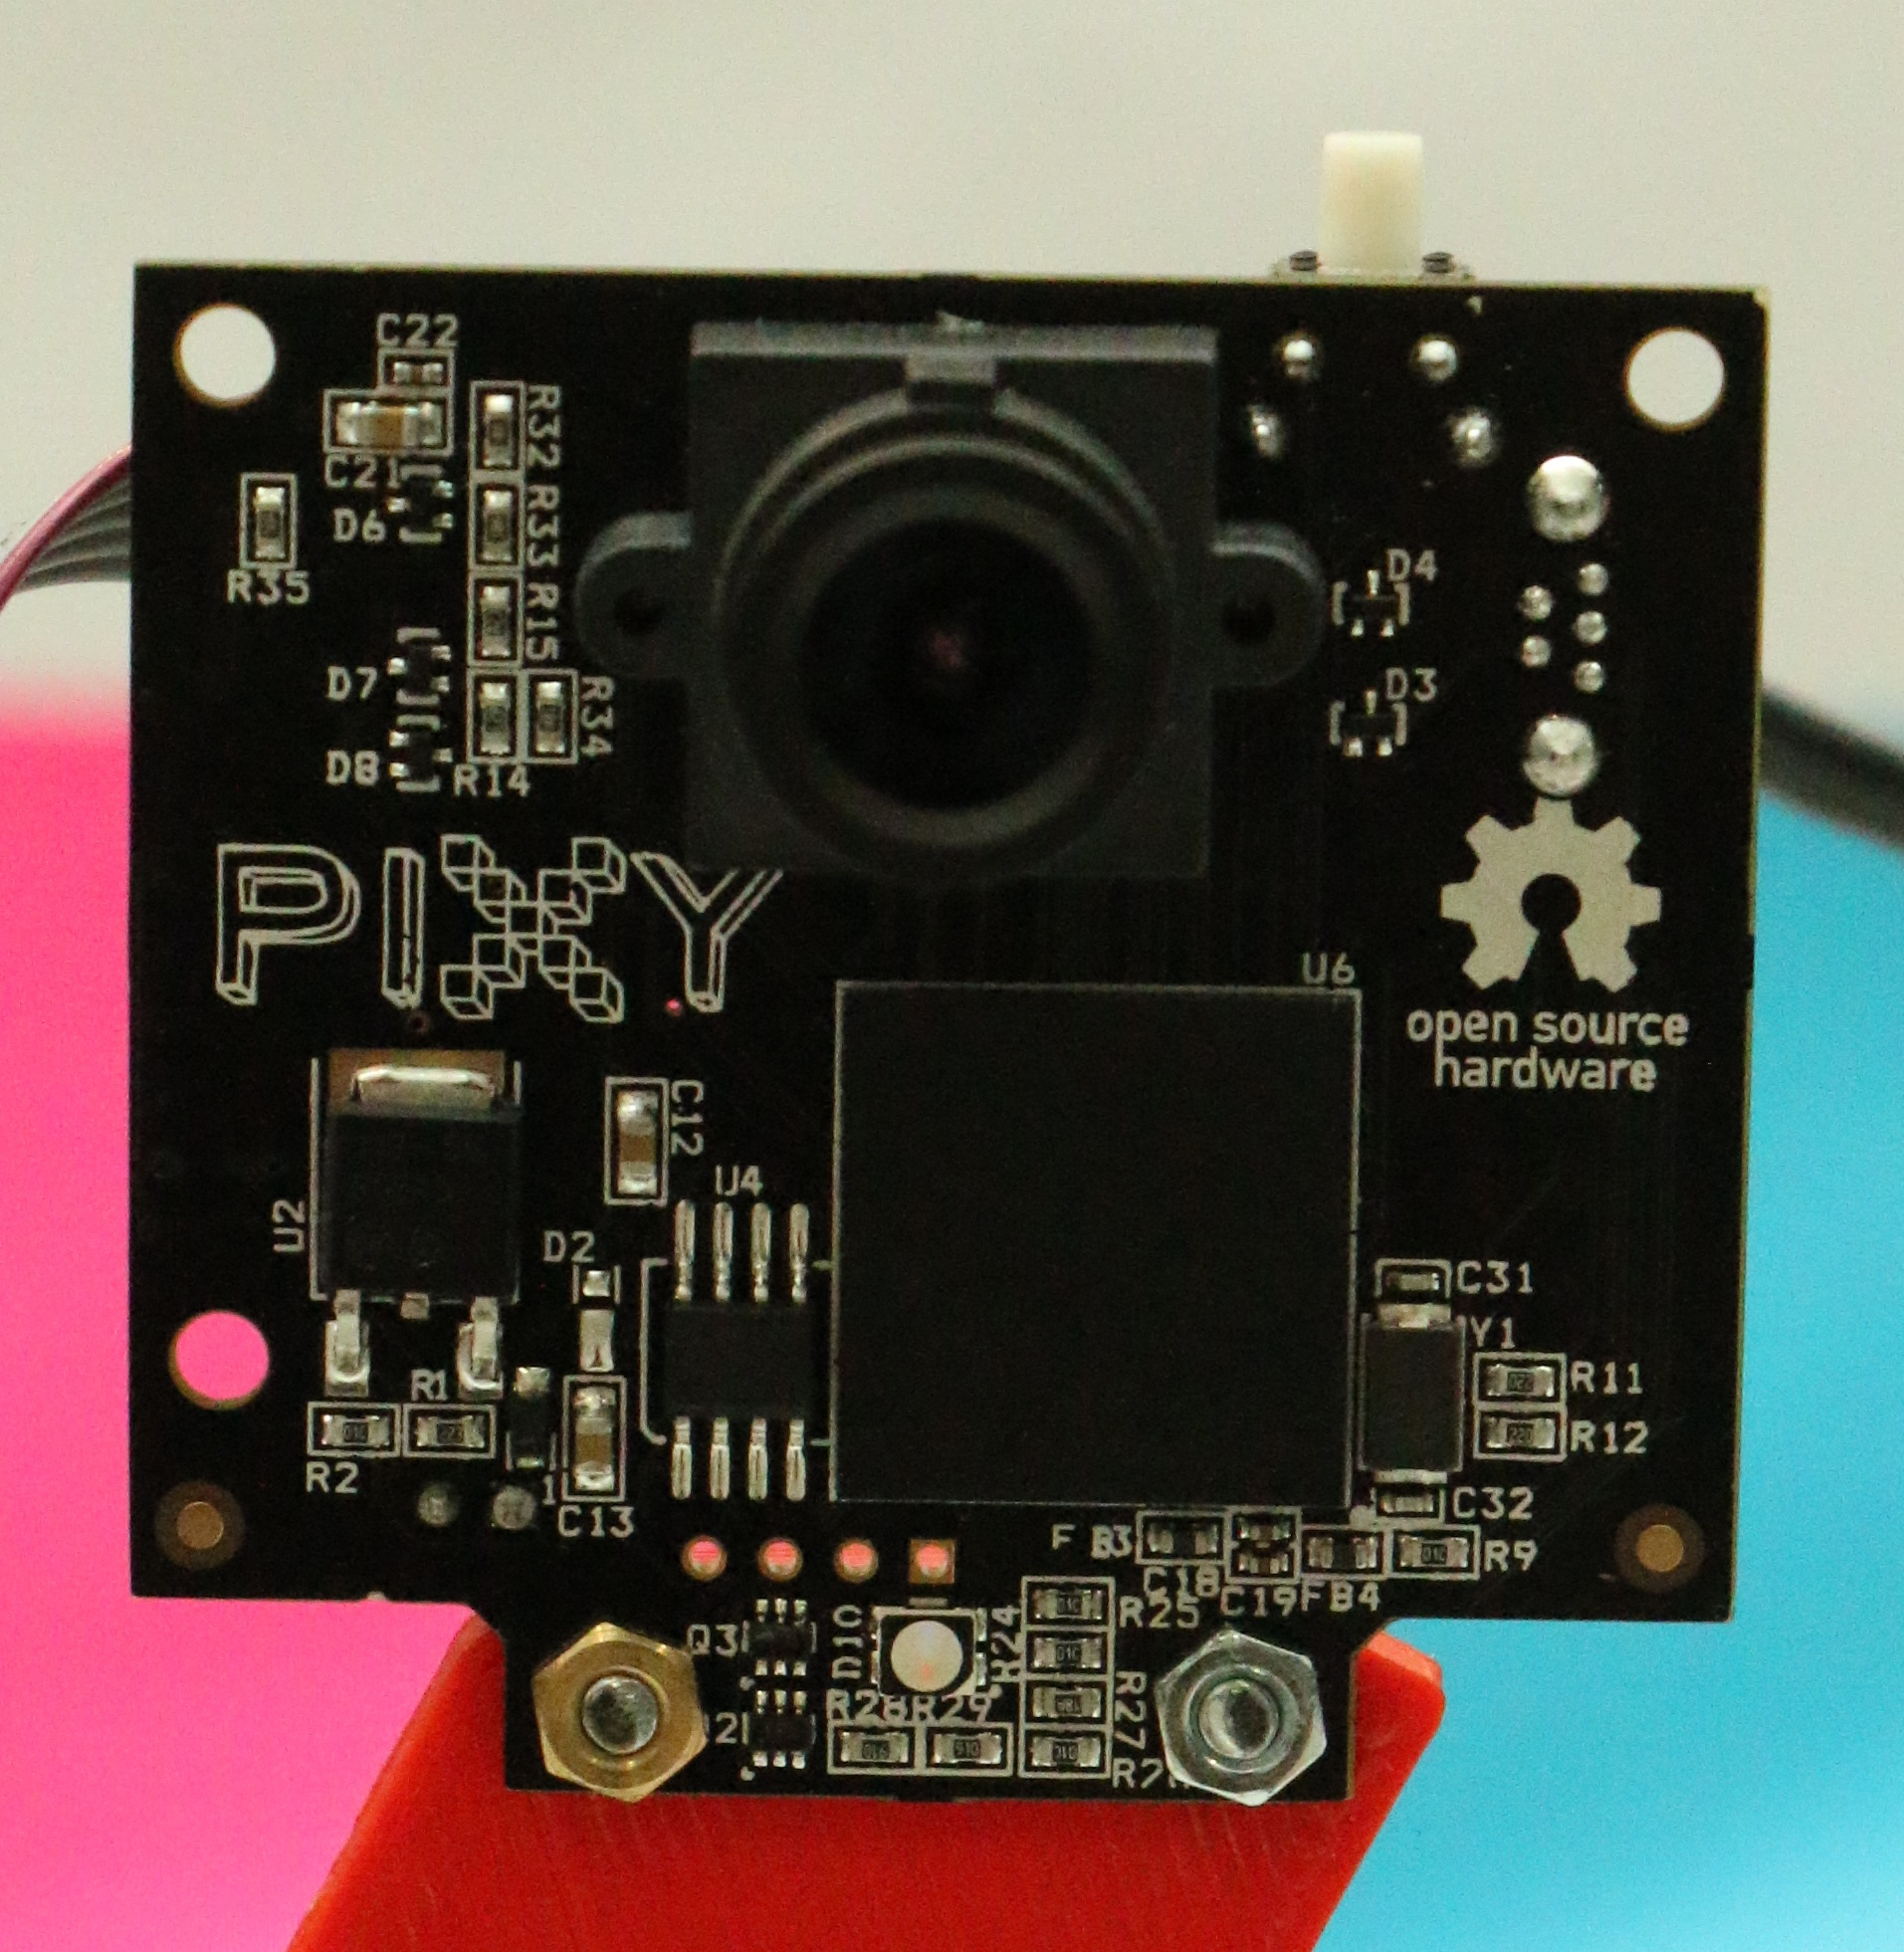
\includegraphics[width = 0.4\textwidth]{Bilder/Pixy_CMUcam5}
  \par\end{centering}
  \caption{PIXY CMUcam5}
  \label{PIXY}
\end{figure}

\begin{figure}[H]
  \begin{centering}
    \subfigure[Colorcode]{
\includegraphics[width = 0.4\textwidth]{Bilder/Colorcode}}
    \subfigure[Objekt]{
\includegraphics[width = 0.4\textwidth]{Bilder/Colorcode}} %%%%%%%%%Objekt statt Colorcode
  \par\end{centering}
  \caption{Erkennbare Objekttypen}
  \label{PIXY_Objekte}
\end{figure}

  \subsection{Technische Planung}
    \subsubsection{Mögliche Verfahren zur Positionserkennung}
    Hier muss grundsätzlich zwischen zwei Messmethoden unterschieden werden:
    \begin{itemize}
      \item \textbf{Absolute Positionsmessung}\\
      Hier wird die Position von einem gleichbleibenden Punkt aus gemessen. Dabei ist ein konstanter Referenzpunkt wichtig.
      Verändert sich dieser oder kann die Distanz nicht genau gemessen werden ist die Messung unbrauchbar.

      Für eine absolute Positionsmessung bieten sich diverse Triangulationsverfahren an,
      diese sind ausgesprochen rechenaufwändig und benötigen meist eine sehr genaue Laufzeitmessung.
      Für die Triangulation können die unterschiedlichsten Signale verwendet werden, am gängigsten sind jedoch jene die mit elektromagnetischen Wellen arbeiten,
      \zB WLAN, Bluetooth. Dies bedeutet, dass sich die Signale mit Lichtgeschwindigkeit ausbreiten.

      Bei einer Messung derart schneller Signale muss ein hoher Aufwand betrieben werden um eine Messgenauigkeit von einigen cm zu erzielen.
      Eine weitere Herausforderung sind Mauern \bzw Hindernisse. Hier muss ständig berücksichtigt werden wo ein Objekt steht und ob der geplante Weg überhaupt frei ist.
      \item \textbf{Relative Positionsmessung}\\
      Hier wird die Position von einem wechselnden Punkt aus gemessen. Um hier eine Positionierung im Raum ermöglichen zu können,
      ist es erforderlich immer zu einem bestimmten Punkt zu messen. Ein Wechsel dieses Punktes ist jedoch möglich,
      deshalb muss auch die Position der Punkte im Raum bekannt sein. Ist die Zielposition im Raum bekannt kann zu dieser hin navigiert werden.
      Auch hier muss wie bei einer absoluten Positionsmessung auf Hindernisse geachtet werden.

      Die zweite Alternative ist, dass eine bestimmte Route bekannt ist und sich das zu positionierende Objekt nur in einem bestimmten Bereich um diese Route bewegt.
      Wird bei der Positionierung der Route bereits auf Hindernisse geachtet müssen diese im Anschluss nicht mehr zwingend beachtet werden.
    \end{itemize}

  \subsection{Umsetzung}
  Durch die PIXY CMUcam5 lässt sich eine relative Positionsmessung vergleichsweise einfach verwirklichen.
  Werden ein oder mehrere Objekte erkannt wird eine bestimmte Nummer (abhängig von der Farbe) sowie die Position am Bild und die Objektgröße übermittelt.
  Die Kamera arbeitet dabei mit einer Bildwiederholrate von 50 Hz, es ist also alle 20 ms eine Auswertung möglich.

  Die Kamera wird auf dem Hexacopter befestigt, mehrere Farbcodes kennzeichnen den Weg zu einem Tisch.
  Um an dieser Stelle eine Navigation zu erreichen wird der Hexacopter so gesteuert, dass er, abhängig von der Route,
  immer einen bestimmten Farbcode betrachtet, ist er über diesem sucht er den nächsten.

    \subsubsection{SPI Schnittstelle}
    Als Schnittstelle für die Kommunikation mit der Kamera wird eine SPI-Schnittstelle verwendet.
    Die Kamera selbst unterstützt unter anderem die seriellen Schnittstellen UART, I2C und SPI.
    Außerdem werden noch ein analoger und digitaler Output unterstütz, diese sind jedoch vergleichsweise beschränkt,
    da keine näheren Informationen zu dem Objekt übermittelt werden können sondern nur die Position \bzw ob überhaupt ein Objekt erkannt wurde.

    Die SPI-Schnittstelle ist bei der Kamera besonders ausfallsicher. Hier wird ein Synchronisationsbyte gefordert, wird dieses nicht erkannt,
    \zB aufgrund eines Fehlers in der Datenübertragung, schickt die Kamera keine Daten.

    \paragraph{Überprüfen der SPI-Schnittstelle}
    Um zu überprüfen ob die SPI-Schnittstelle auch korrekt arbeitet wird bei der ersten Inbetriebnahme der Output überprüft.
    Hierzu wird der Zustand der 3 Leitungen mit einem Oszilloskop betrachtet.
    \begin{itemize}
      \item \textcolor{blue}{Taktleitung}
      \item \textcolor{red}{Dateneingang (PIC)}
      \item \textcolor{green}{Datenausgang (PIC)}
    \end{itemize}

    \begin{figure}[tbh]
      \begin{centering}
        \subfigure[Großer Zeitbereich]{\includegraphics[width = 0.49\textwidth]{Bilder/SPI_gross}}
        \subfigure[Kleiner Zeitbereich]{\includegraphics[width = 0.49\textwidth]{Bilder/SPI_klein}}
      \par\end{centering}
      \caption{Ausgang der SPI Schnittstelle}
      \label{SPI-Ausgang}
    \end{figure}

    Der Wert mit dem diese Überprüfung durchgeführt wird sollte möglichst variabel sein, hier wird 0xAA (1010 1010) verwendet.
    Wird dieser Wert nicht variabel angenommen kann es dazu kommen, dass fälschlicher Weise angenommen wird, dass die Übertragung korrekt ist.
    Der Dateneingang des PIC, respektive der Ausgang der Kamera, zeigt eine deutliche Störung durch die Taktleitung an.

    \subsubsection{Erkennen und Auswerten eines Bildes}
    Die Kamera schickt der Reihe nach die einzelnen Daten eines Objekts. Darunter ist auch eine Startbedingung welche ein neues Bild markiert.
    Mit den diversen Informationen zum Objekt ergeben sich folgende Daten:
    \begin{itemize}
      \item Neues Bild 0xAA55
      \item Objekt 0xAA55 oder Farbcode 0xAA56
      \item Checksum
      \item Objektnummer
      \item X-Position
      \item Y-Position
      \item Breite
      \item Höhe
      \item Drehwinkel, nur bei Farbcodes
    \end{itemize}
    Dabei ist die Objektnummer von den im Objekt oder Farbcode vorkommenden Farben abhängig, zusätzlich ist zu beachten, dass sie oktal dargestellt wird.
    Ein übermittelter Wert von dezimal 10, also oktal 12, bedeutet, dass die Farben 1 und 2 erkannt wurden.

    Will man nun ein neues Bild finden muss man so lange nach 0xAA55 suchen bis man diese Daten gesendet bekommt.
    Anschließend gilt es noch festzustellen ob man einen Farbcode oder ein Objekt betrachtet,
    es muss also direkt darauf 0xAA56 oder nochmals 0xAA55 erkannt werden. Ist dies nicht der Fall, wurde kein neues Bild erkannt und man betrachtet ein normales Objekt.

    Betrachtet man nun die bis zum Erkennen eines neuen Bildes gesendeten Daten als gegenstandslos ergibt sich eine vergleichsweise einfache Schleife um ein Bild zu erkennen.

    \lstset{language = c}
    \begin{lstlisting}
while(frame == 0) {
  w = ExchangeSpiWord(PIXY_SYNC, DUMMY);
  if(lw == PIXY_FRAME_OBJ && w == PIXY_FRAME_OBJ) {
    frame = 1;
    obj_type = 0;
    a_color[c_obj].type = PIXY_FRAME_OBJ;
  } else if(lw == PIXY_FRAME_OBJ && w == PIXY_COLORCODE) {
    frame = 1;
    obj_type = 1;
    a_color[c_obj].type = PIXY_COLORCODE;
  } else if(w == 0 && lw == 0){
    frame = 0;
  }
  lw = w;
  c++;
  if(c > 254) {
    return 0;	//****Error, end of function
  }
}
    \end{lstlisting}
    Um nicht ewig in dieser Schleife fest zu hängen, wenn kein Bild erkannt wird und einen Fehler auslösen zu können wird die gesamte Funktion der Bildauswertung
    nach 255 Versuchen verlassen.

    Die weiteren Werte eines Objekts werden der Reihe nach in einer Structur abgespeichert, hier ist nichts besonderes mehr zu beachten.

  \subsection{Herausforderungen und Lösungen}

%%%%%%%%%%%%%%%%%%%%%%%%%%%%%%%%%%%%%%%%%%%%%%%%%%%%%%%%%%%%%%%%%%%%%%%%%%%%%%%
\section{Ultraschallsensor HC-SR04}
Der Ultraschallsensor HC-SR04 ist ein für Arduino entwickeltes Modul um Abstände zu messen. Die Messung geschieht durch das Aussenden von Ultraschallimpulsen,
die Messgröße wird dabei als laufzeitabhängiger Impuls retourniert.

\begin{figure}[tbh]
  \begin{centering}
    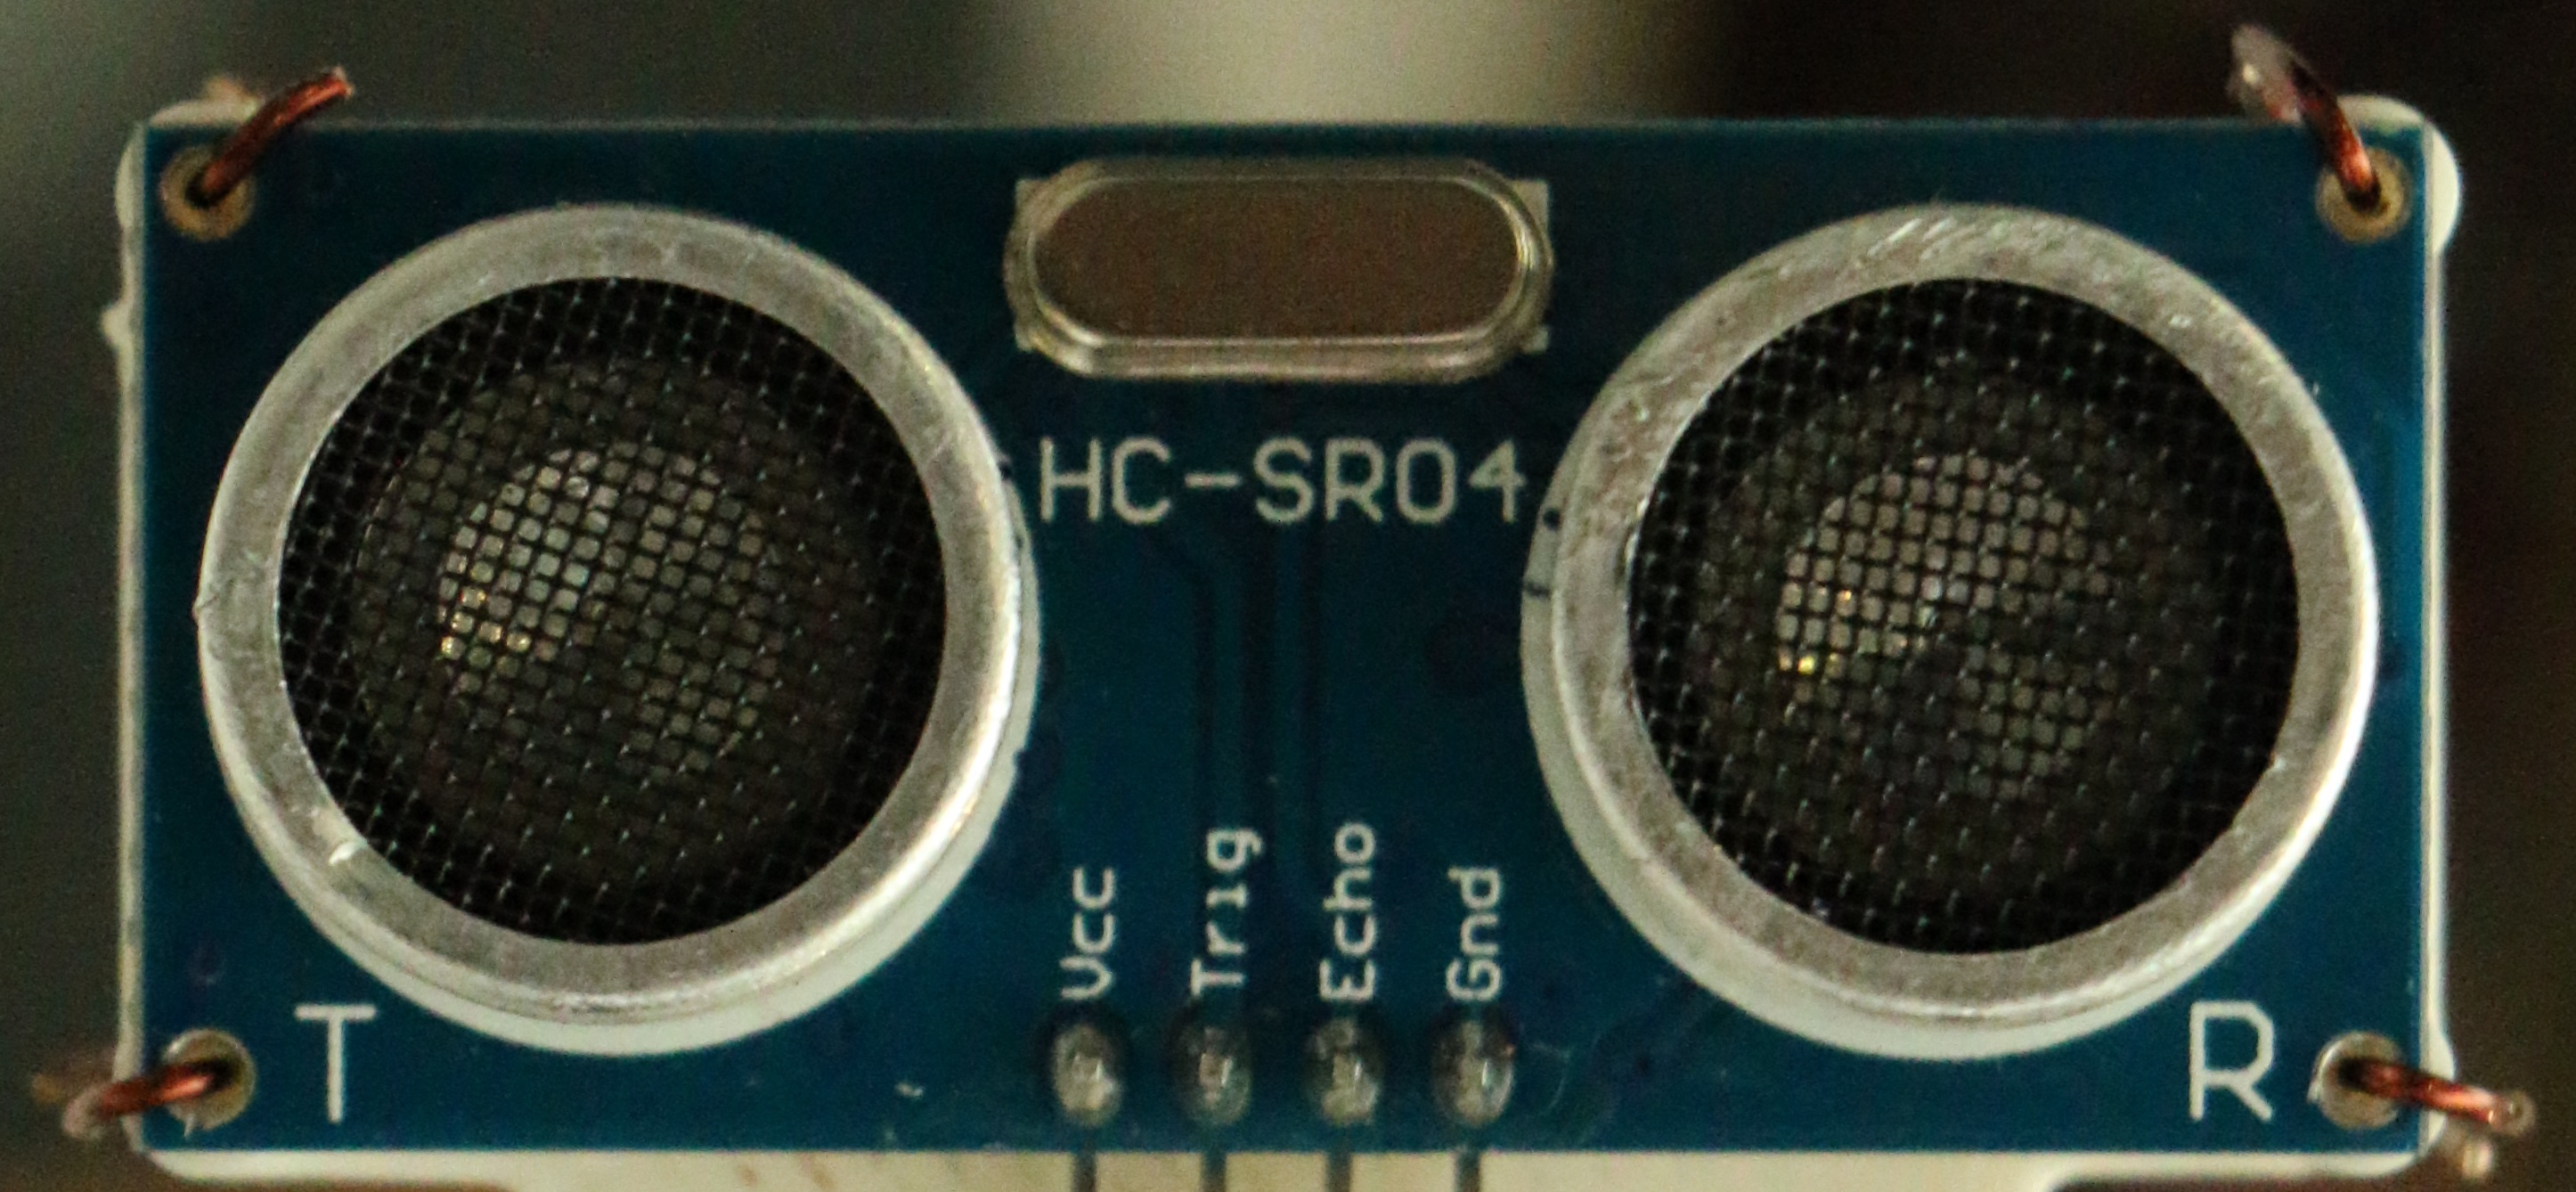
\includegraphics[width = 0.5\textwidth]{Bilder/Ultraschallsensor}
  \par\end{centering}
  \caption{Ultraschallsensor HC-SR04}
  \label{Ultraschallsensor}
\end{figure}

  \subsection{Technische Planung}
  Für die Steuerung des Hexacopter ist es notwendig die aktuelle Flughöhe zu wissen.
  Es ist mit einer bekannten Objektgröße und den von der Kamera vorliegenden Daten zwar möglich die aktuelle Flughöhe rechnerisch zu bestimmen,
  jedoch gestaltet sich dies sehr rechenaufwändig. Um die Höhe möglichst einfach messen zu können bietet sich daher eine vergleichsweise langsame Messung,
  wie jene mit einem Ultraschallsignal an.
  Bei einer Schallgeschwindigkeit von $\SI{343}{\meter\per\second}$ entstehen bei einer zu messenden Distanz von $\SI{2}{\meter}$,
  Laufzeiten des Ultraschallsignals von \ca $\SI{12}{\milli\second}$ (Distanz mal 2 da das Signal wieder zurückkehren muss).

  \subsection{Umsetzung}
  Abhängig von der mit dem Mikroprozessor ermittelten Laufzeit $time\_height$ lässt sich jederzeit die aktuelle Flughöhe bestimmen.
  \[
  s(time\_height) = \frac{v \cdot t}{2} = \frac{\SI{343}{\meter\per\second} \cdot time\_height}{2}
  \]
  Die Höhe wird dabei in der main-Routine durch den Aufruf folgender Funktionen regelmäßig bestimmt:
  \lstset{language = c}
  \begin{lstlisting}
void StartHeightMeasure(void) {
  TMR5L = 0;
  TMR5H = 0;
  Trigger = 0;
}

void ReadHeight(void) {
  while(TMR5GIF == 0);
  TMR5GIF = 0;
  time_height = 0;
  time_height = TMR5H;
  time_height <<= 8;
  time_height |= TMR5L;
  TMR5L = 0;
  TMR5H = 0;
  a_frame[0].height = time_height;
  a_frame_dif[0].dif_height = a_frame[1].height - a_frame[0].height;
  Trigger = 1;
}
  \end{lstlisting}

  In der ersten Funktion wird die Messung gestartet. Dazu wird ein Trigger-Signal an den Ultraschallsensor gesendet, dieser reagiert auf eine fallende Flanke.
  Zuvor wird darauf geachtet, dass die Register in denen die Zeit zurückgegeben wird auch wirklich leer (= 0) sind.
  In der zweiten Funktion folgt das Auslesen der vorhandenen Daten. Dazu werden die zwei 8-Bit Register in der 16-Bit Variable $time\_height$ abgespeichert.
  Zusätzlich wird die gemessene Höhe für die Auswertung in der $a\_frame[0].height$ Variable abgespeichert und die Differenz zur vorhergehenden Messung ermittelt.

  Auf eine Berechnung der genauen Höhe in m wird zu Gunsten der Verarbeitungszeit verzichtet, auf die spätere Auswertung der Flugdaten hat dies keinen Einfluss.

  \subsection{Herausforderungen und Lösungen}
  \textcolor{red}{to be continued after realtime measurements}

\chapter{Aktoren}
\renewcommand{\kapitelautor}{Autor: Lucas Ullrich}

%%%%%%%%%%%%%%%%%%%%%%%%%%%%%%%%%%%%%%%%%%%%%%%%%%%%%%%%%%%%%%%%%%%%%%%%%%%%%%%
\section{Propeller, A E T und R}

  \subsection{Technische Planung}

  \subsection{Umsetzung}

  \subsection{Herausforderungen und Lösungen}


% !TEX root = diplomarbeit.tex
\chapter{Firmware}
\renewcommand{\kapitelautor}{Autor: Christina Bornberg, Lucas Ullrich}

%%%%%%%%%%%%%%%%%%%%%%%%%%%%%%%%%%%%%%%%%%%%%%%%%%%%%%%%%%%%%%%%%%%%%%%%%%%%%%%
\section{Allgemeine technische Planung}

  \subsection{Programmiersprache}
  Zum Programmieren des Mikrocontrollers wurde die Programmiersprache C verwendet.

  \subsection{Tools}

    \begin{itemize}
      \item \textbf{yEd - Graph Editor}\\
      Zum erstellen der benötigten Flussdiagramme wurde eine Desktop Anwendung namens yEd verwendet.
      \item \textbf{GitHub}\\
      Zur Versionsverwaltung des Codes wurde die digitale Ablage GitHub verwendet. Durch diese ist eine gemeinsame Programmierung möglich.
      \item \textbf{MPLAB}\\
      MPLAB ist eine Integrierte Entwicklungsumgebung von Microchip. In dieser wurde der Mikrocontroller programmiert und anschließend das C-Programm in Assembler compiliert.
      Weiters hat die Entwicklungsumgebung eine Git Funktion, wodurch die Daten ohne zusätzliches Tool vom Server herunter- beziehungsweise hinaufgeladen werden können.
    \end{itemize}


  \subsection{Positionierungssystem - evtl an anderen Ort}

    \subsubsection{Anwendung}
    Indoor Positionierungssysteme werden derzeit vor allem zum Objekterkennung, im Umweltmonitoring, über das Detektieren von Bränden in Gebäuden,
    bis hin zum Einsatz in der Logistik verwendet. Da es sehr viele unterschiedliche Anwendungsgebiete gibt, werden unterschiedliche Methoden verwendet.

    \subsubsection{Art der Positionsbestimmung}

    Ein Lokalisierungssystem kann verschiedene Arten von Informationsdaten bereitstellen. Es gibt dazu physische, symbolische, absolute und relative Modelle.

      \begin{itemize}
        \item \textbf{Physische Positionierung}\\
        Die physische Positionierung wird in Form von Koordination bestimmt, meist in 2-D oder 3-D Karten. Längen- und Breitengrade spielen dabei eine wichtige Rolle.
        \item \textbf{Symbolische Positionierung}\\
        Symbolische Positionierung wird sprachlich beschrieben, wie \zB Küche, Keller usw.
        \item \textbf{Absolute Positionierung}\\
        Die absolute Positionierung verwendet Referenzgitter und Koordinaten. Das Paradebeispiel für absolute Ortung ist die Angabe von Längen­ und Breitengrad.
        Die darauf aufsetzende Technik, die sich diese Kartographie zu Nutze macht, ist GPS.
        \item \textbf{Relative Positionierung}\\
        Die relative Positionierung verwendet legt ihre eigenen Rahmen vor, die auf Basisstationen oder definierten Punkten basieren.
        Anders als bei der absoluten Lokalisierung muss bei der relativen Positionsbestimmung die vorherige Position des Objektes bekannt sein, auf die wird dann die Position bezogen.
      \end{itemize}


    \subsubsection{Selbst- und fernortende Lokalisierungstechniken}

    Lokalisierungstechniken können weiter als selbstortend oder fernortend (engl. self­positioning/remote­positioning) klassifiziert werden.

    Fernortende Positionierungssystem: Mobile, bewegliche Sender mit stationären, unbeweglichem Empfänger. Die Messdaten aller Empfänger werden gesammelt und die
    Position des Senders wird in der Zentrale berechnet. Hier ist ein Netzwerk notwendig, sämtliche Berechnungen werden durch eine zentrale Instanz ausgeführt.

    Selbstortende Positionierungssystem: Der mobile, bewegliche Empfänger bekommt die Daten von verschiedenen Sendern, die sich auf bekannten Positionen befinden.
    Die Lokalisation des Empfängers wird durch die gemessenen Signale ermittelt. Das Objekt kann sich selbst orten, es ist kein Netzwerk notwendig.



    \subsubsection{Algorithmen}

    Prinzipiell gibt es vier Möglichkeiten, eine Positionierung vorzunehmen.
    \begin{itemize}
      \item Lateration, also die Bestimmung der Position mit Hilfe von Entfernungsmessungen
      \item Angulation, hier werden Winkelmessungen zu Hilfe genommen
      \item Szenenanalyse, bei der Umgebungsparameter erfasst und ausgewertet werden
      \item Nachbarschaft (engl. proximity) bei der physische Nähe ausgenutzt wird.
    \end{itemize}

    Die dahinterstehenden Algorithmen basieren auf den Methoden der Bestimmung von Distanzen, Winkelen, Dreiecken und Nachbarschaften.

    Können die ermittelten Informationen auch mit einer vorher bestimmten Radio-Map verglichen werden bezeichnet man dieses Verfahren auch Fingerprinting.



    \subsubsection{Funktechnik}
    % die Tabelle in rosa :b %


    \textbf{Technologien}\\
    \begin{itemize}
        \item \textbf{GPS}\\
        OUTDOOR
        \item \textbf{RFID}\\
        \item \textbf{WPS}\\
      \end{itemize}

    \subsubsection{Optisches Tracking}

    \textbf{Pixy CMUcam5}\\




  \subsection{Konzepte}
  Die verschiedenen Positionierungsarten wurden verwendet, um Konzepte für die Navigation zu entwickeln.

    \subsubsection{Aufgabenstellung}
    Damit der Hexacopter autonom durch den Raum navigieren kann, benötigt er ein Positionierungssystem.

    \subsubsection{Funkbasiertes Tracking}

      \textbf{Tracking mittels Signalstärke}\\

      % Das vom John ???

      Nachteile:
      Muss sehr präzise sein.
      Störungen durch andere elektromagnetische Wellen im selben Frequenzbereich.



      \textbf{Tracking mittels Laufzeitmessung}\\

      % Durch ein künstlich erstelltes lokales GPS


      % Fraunhofer: Mit Hilfe der Laufzeitmessung werden Objekte (Gegenstände oder Personen), welche mit kleinen Tags ausgestattet sind, geortet. Dazu werden Signale zwischen Sendern und Empfängern verschickt. Je nachdem, ob das Signal lange oder kurze Zeit benötigt, ist der Gegenstand weit entfernt oder ganz nah. Dies funktioniert, da man weiß, dass sich elektromagnetische Wellen mit Lichtgeschwindigkeit ausbreiten. Wird die Lichtgeschwindigkeit c mit der gemessenen Laufzeit multipliziert, kann die genaue Entfernung berechnet werden. Die Laufzeit kann mit unterschiedlichen Messprinzipien bestimmt werden, zum Beispiel mittels extrem kurzer UWB-Impulse (Ultrawideband) oder auch mit Hilfe von Korrelationsalgorithmen, die die Bekanntheit von Signalsequenzen nutzen.


    \subsubsection{Optisches Tracking}
    % Aufgrund der Komplexität einer signalbasierten


      \textbf{Kamerasystem im Raum}\\
      Verteilte Kameras in einem Raum tracken den Hexacopter mittels Marker. Dadurch kann die Position des Hexacopters bestimmt werden.


      \textbf{Linien}\\
      Zunächst wurde ein Konzept mit Linien erstellt. Der Hexacopter folgt einer einfarbigen Linie, bis er zu einer Kreuzung kommt, nun ist seine Aufgabe, die nächste Linie zu finden, um seinen Weg zum Ziel zu finden.

      Vorteile: Der Hexacopter kann die Linie nur schwer verlieren
      Nachteile: Das verwendete Kamerasystem ist nicht in der Lage eine Linie zu tracken.

      \textbf{Tracking mittels Infrarot}\\


      Vorteile:
      System funktioniert ebenfalls im Dunkeln.
      Nachteile:
      Jeder Tisch benötigt einen Stromanschluss.
      Die Wartung ist aufwändig.

      \textbf{Farbcode pro Wegabschnitt}\\
      Durch die Verwendung der Pixy CMUCam5 ergibt sich die Möglichkeit, Farbobjekte, die eine oder mehrere Farben haben, zu scannen.



      \textbf{Farbcodes variieren}\\
      Das gewählte System wird ebenfalls mittels 2-farbiger Codes umgesetzt.


      relative Positionierung ist ausreichend

      Vorteile:
      keine großartigen Kosten neben Copter und Server
      Rechnung am Hexacopter

      Nachteile:
      Aufwand im Restaurant



  \subsection{Tischkonzept}

  % Bild vom Ablauf %%%%%%%%%%%%%%%%%%%%%%%%%%%%%%%%


  \subsection{Flussdiagramme}
  Für einen besseren Überblick über die einzelnen Programme und deren geforderten Funktionen wurden einzelne Flussdiagramme des gesamten Prozesses erstellt.
  Diese dienen nachfolgend als Orientierung beim Programmieren der einzelnen Funktionen.

  \begin{figure}[tbh]
    \begin{centering}
      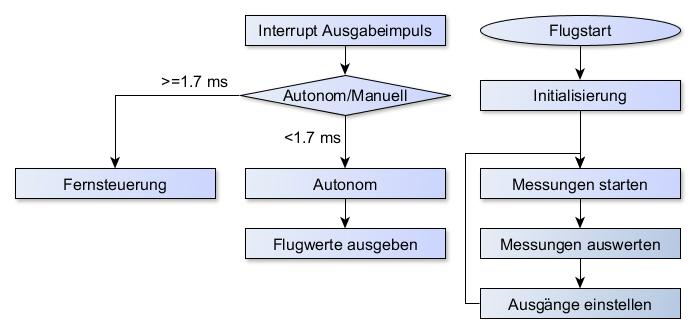
\includegraphics[width = \textwidth]{Bilder/Flussdiagramm}
    \par\end{centering}
    \caption{Flussdiagramm des Gesamtablaufs}
    \label{Flussdiragramm}
  \end{figure}

  Für die weiteren Programmteile wurden jeweils noch detailliertere Flussdiagramme erstellt.

  \subsection{Aufbau des Programms}

  % Erklärung, wer was Aufruft %





%%%%%%%%%%%%%%%%%%%%%%%%%%%%%%%%%%%%%%%%%%%%%%%%%%%%%%%%%%%%%%%%%%%%%%%%%%%%%%%
\section{Navigation}

  \subsection{Technische Planung}



    \subsubsection{Frames}

    % BILD VON LUCAS %


    \subsubsection{Aileron}
    \subsubsection{Elevator}
    \subsubsection{Rudder}

    % Rotationsbild + 2er Komplement %

    \subsubsection{Throttle}

  \subsection{Umsetzung}

    \subsubsection{Vergleichen der Frames}
    Für den Vergleich des aktuellen mit dem letzten Frame, werden zwei \glslink{Struktur}{Strukturen} verwendet, die über folgende Mitglieder verfügt.
    \begin{itemize}
      \item \textbf{num}\\
      ist die ID des getrackten Colorcodes, er besteht aus einer zweistelligen Zahl.
      \item \textbf{pos\_x}\\
      ist die X-Position des Colorcodes. Der Wert bezieht sich auf das Zentrum des Objektes.
      \item \textbf{pos\_y}\\
      ist die Y-Position des Colorcodes. Der Wert bezieht sich auf das Zentrum des Objektes.
      \item \textbf{height}\\
      ist die, vom Ultraschall übergebene Höhe.
      \item \textbf{angle}\\
      ist die Rotation des Colorcodes. Da er zweifarbig ist, kann die PIXY CMUcam5 die Rotation des Objektes feststellen.
    \end{itemize}

    Quelle: \textcolor{red}{TITEL FEHLT \cite{Structs}, das sollte verlegt werden -Lucas}

    Zuerst wird die ID des Colorcodes verglichen, um herauszufinden, ob das Farbobjekt das selbe wie im letzten Frame ist.
    Sollte dies der Fall sein, werden die Koordinaten x und y und die Rotation mit den Werten der älteren Struktur verglichen und gespeichert.
    Diese werden bei den folgenden Funktionen verwendet, um zu überprüfen, ob der Hexacopter die richtige Geschwindigkeit hat.

    \subsubsection{Aileron, Elevator und Rudder anhand der Kameradaten}
    Durch die PIXY CMUcam5 kann die Position des Hexacopters, relativ zu einem Colorcode, festgestellt werden. Gegebenenfalls werden anschließend die Flugparameter verändert.

    \begin{figure} [tbh]
      \begin{centering}
        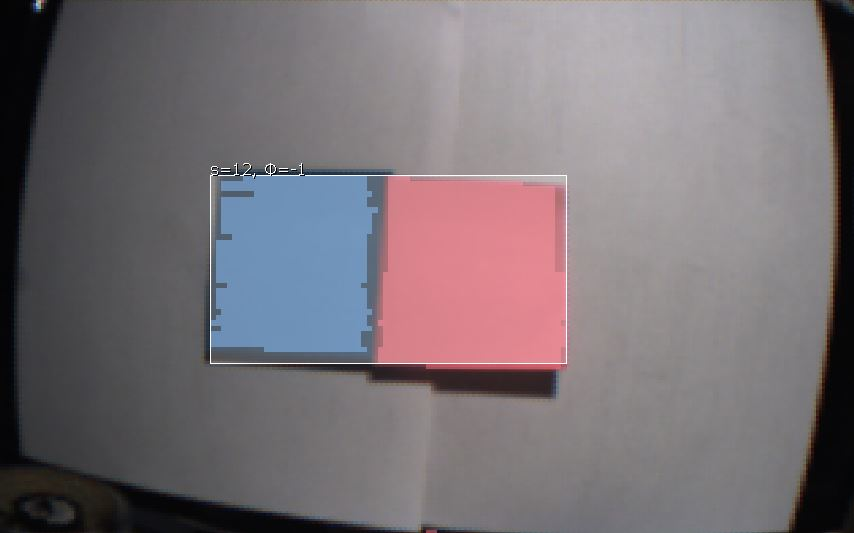
\includegraphics[width = \textwidth]{Bilder/Farbcode_erkannt}
      \par\end{centering}
      \caption{Ein erkannter Farbcode}
      \label{Farbcode_erkannt}
    \end{figure}
    Die Position wird anhand solcher Farbcodes erkannt, im Tischkonzept ist hinterlegt in welcher Reihenfolge der Hexacopter die Farbcodes suchen muss.
    Er fliegt anschließend so lange, bis er über dem aktuellen Farbcode ist, dieser also mittig im Bild ist und sucht darauf den nächsten.


    Die PIXY CMUcam5 XXXXXX % IRGENDWAS MIT X diese länge, y diese länge; %



      \begin{itemize}
        \item \textbf{Überprüfen von Aileron}\\
        Die Überprüfung von Aileron bezieht sich auf die Beschleunigung nach Links und Rechts, was der x-Koordinate entspricht.

        Ziel der Funktion ist es, den Farbcode in die Mitte des Frames zu bekommen. Der Idealzustand befindet sich zwischen 150 und 170.
        Sollte dieser Zustand erreicht werden, bleibt der Wert von Aileron unverändert und der Hexacopter fliegt weiterhin mit einer unveränderten Beschleunigung an der
        x-Koordinate.
        Sollte dies nicht der Fall sein, muss der Wert auf einige Komponenten \textcolor{red}{XXXXX} überprüft werden.
        Wenn der Farbcode zu weit auf der rechten Seite liegt, das bedeutet, wenn der Wert des Mittelpunktes vom Farbobjekt höher als 170 ist,
        muss der Hexacopter nach rechts fliegen, um seine Position zu korrigieren.
        Dabei muss zuerst verglichen werden, ob sich der Hexacopter in die richtige Richtung bewegt. Sollte er in die falsche Richtung
        fliegen, wird der Aileron-Flugparameter gesenkt, dies setzt die Beschleunigung nach Rechts vorraus.
        Wenn die Beschleunigung nach rechts hoch genug ist und die Drohne tatsächlich nach rechts fliegt, wird die Geschwindigkeit überprüft.
        Die Geschwindigkeit wird durch die Differenz der x-Koordinate beider Strukturen herausgefunden. Die Einheit ist in diesem Fall

        \item \textbf{Überprüfen von Elevator}\\
        Position der Farbobjekte (CHECK AILERON \& ELEVATOR)
        Wenn ein Farbobjekt nicht im gewünschten Bereich plaziert ist, muss der Hexacopter weiter nach links oder weiter nach rechts fliegen.
        \item \textbf{Überprüfen von Rudder}\\
        Rotation der Farbojekte (CHECK RUDDER)
        Wenn der Hexacopter über einem Farbobjekt fliegt, soll er kontrollieren, ob der 2-Farbige Code die richtige Rotation hat und sich im richtigen Bereich des Bildschirmes befindet. Wenn diese Informationen richtig sind, darf der Copter zum nächsten Farbobjekt fliegen.
        Durch dieses System könne die genauen Wege vorgegeben werden und können sich durch das gesamte Restaurant verteilen. Durch die Rotation der Codes können auch Kurven eingebaut werden.

        Richtung (CHECK RUDDER)
        Durch die Rotation der Colorcodes, kann der Hexacopter bestimmen, ob er den richtigen Weg und in die richtige Richtung fliegt, wenn er am Weg zurück zur Base ist, muss er den umgekehrten Colorcode verwenden. (Rotation 180Grad)
      \end{itemize}

    \subsubsection{Throttle anhand des Ultraschallsensors}

    Starten und landen auf Landeplattformen (CHECK THROTTLE)
    Der Hexacopter startet und landet auf den mit ebenfalls mit Colorcodes gekennzeichneten Landeplattformen.
    Bei einem Fehler, besteht auch das Landen auf einem beliebigen Fleck

    Höhe korrigieren (CHECK THROTTLE)
    Höhenunterschied zwischen Tisch und Boden

    \subsubsection{Speichern der alten Daten}

    \subsubsection{Ausgabe der Steuersignal}
    Nachdem die Steuersignale berechnet und korrigiert wurden müssen diese an den Hexacopter ausgegeben werden. Dies muss periodisch alle $\SI{20}{\milli\second}$ geschehen.
    Der Flightcontroller erkennt jeweils die einzelnen Impulse und steuert die Rotoren entsprechend an.

    Diese Impulse werden Interrupt-gesteuert ausgegeben, der Interrupt wird von dem Gear-Pin erzeugt welcher gleichzeitig für den Flugmodus verantwortlich ist.

    \lstset{language = c}
    \begin{lstlisting}
interrupt void Isr() {
  if(CCP1IF == 1) {
    CCP1IF = 0;
    T1CONbits.TMR1ON = 0;
    SignalOut();
    NOP();
  }
  if(TMR3GIF == 1) {
    TMR3GIF = 0;
    ModeCheck();
    SignalOut();    /* initial call after remaining break to 20 ms
                     * starts with Aileron (needs to be set in last
                     * case statement, case 0) following delays will
                     * be processed by the previous routine */
    pulsecounter++;
  }
}

void SignalOut(void) {
  switch(pin_out) {
    case 'A': {
      A = 1;
      Delay(a_actors[0].aile);
      pin_out = 'E';
      break;
    }case 'E': {
      A = 0;
      E = 1;
      Delay(a_actors[0].elev);
      pin_out = 'T';
      break;
    }
    \end{lstlisting}
    Die weiteren Signale (Throttle und Rudder) werden auf die gleiche Weise ausgegeben.
    Die Delay-Funktion stellt die Compare-Einehit so ein, dass nach der gewünschten Pulsdauer des Ausgangs ein Interrupt hervorgerufen wird.

%%%%%%%%%%%%%%%%%%%%%%%%%%%%%%%%%%%%%%%%%%%%%%%%%%%%%%%%%%%%%%%%%%%%%%%%%%%%%%%
\section{Objekterkennung}

  \subsection{Technische Planung}

  \subsection{Umsetzung}

  \subsection{Herausforderungen und Lösungen}

%%%%%%%%%%%%%%%%%%%%%%%%%%%%%%%%%%%%%%%%%%%%%%%%%%%%%%%%%%%%%%%%%%%%%%%%%%%%%%%
\section{Sicherheit}

  \subsection{Technische Planung}

  \subsection{Umsetzung}

  \subsection{Herausforderungen und Lösungen}

%%%%%%%%%%%%%%%%%%%%%%%%%%%%%%%%%%%%%%%%%%%%%%%%%%%%%%%%%%%%%%%%%%%%%%%%%%%%%%%
\section{Systemausfall}

  \subsection{Technische Planung}

  \subsection{Umsetzung}

  \subsection{Herausforderungen und Lösungen}


% !TEX root = diplomarbeit.tex
\chapter{Kommunikation Applikation und Hexacopter}
\renewcommand{\kapitelautor}{Autor: Katharina Joksch, Lucas Ullrich}
Um zwischen dem Hexacopter und dem Server eine Verbindung herzustellen wird eine Kommunikationsschnittstelle benötigt. Diese muss Drahtlos arbeiten und einen größeren Bereich
abdecken. Über diese werden anschließend die diversen Daten übertragen, dazu zählen \zB die Route, \bzw der Name des Gastes.

%%%%%%%%%%%%%%%%%%%%%%%%%%%%%%%%%%%%%%%%%%%%%%%%%%%%%%%%%%%%%%%%%%%%%%%%%%%%%%%
\section{Allgemeine technische Planung}
In der Planung wurde eine unkomplizierte und verlässliche Lösung für beide Kommunikationspartner gesucht. Da Bluetooth kaum noch standardmäßig verbaut wird hier wiederum
Serverseitig eine externe Hardware benötigt, um dies zu vermeiden wurde WLAN ins Auge gefasst.

WLAN stellte sich folglich als ideale Schnittstelle heraus,
es gibt die Möglichkeit zu Handover in sehr großen Bereichen, es ist nach einmaligem Setup vergleichsweise unkompliziert und es bietet diverse Möglichkeiten um festzustellen
ob die Verbindung noch aufrecht ist.

%%%%%%%%%%%%%%%%%%%%%%%%%%%%%%%%%%%%%%%%%%%%%%%%%%%%%%%%%%%%%%%%%%%%%%%%%%%%%%%
\section{Schnittstelle Hexacopter}
Seitens des Hexacopters wird ein zusätzliches Modul benötigt, dieses muss über eine der Schnittstellen des Mikrocontrollers ansprechbar sein.

  \subsection{Technische Planung}
  Bei der Planung wurde darauf geachtet ein WLAN-Modul zu wählen welches bekannter maßen funktioniert \bzw ein entsprechender Support zur Verfügung steht.
  So fiel die Wahl auf das WLAN-Modul RN171, vertrieben durch Microchip, hergestellt von Roving Networks.

  Das gewählte WLAN-Modul wird über eine UART-Schnittstelle angesteuert und verfügt über einige frei konfigurierbare Pins, diese werden schließlich zum Überwachen der
  Verbindung verwendet.

  \subsection{Umsetzung}
  Bei der Umsetzung stand für die anfänglichen Tests ein Evaluation-Kit zur Verfügung. Dieses kann ohne weitere Hardware direkt über ein USB-Kabel mit einem PC verbunden werden.
  So ist es möglich die nötigen Konfigurationen des Moduls auszutesten bevor dieses in der Hardware implementiert wird.

  \begin{figure}[H]
    \begin{centering}
      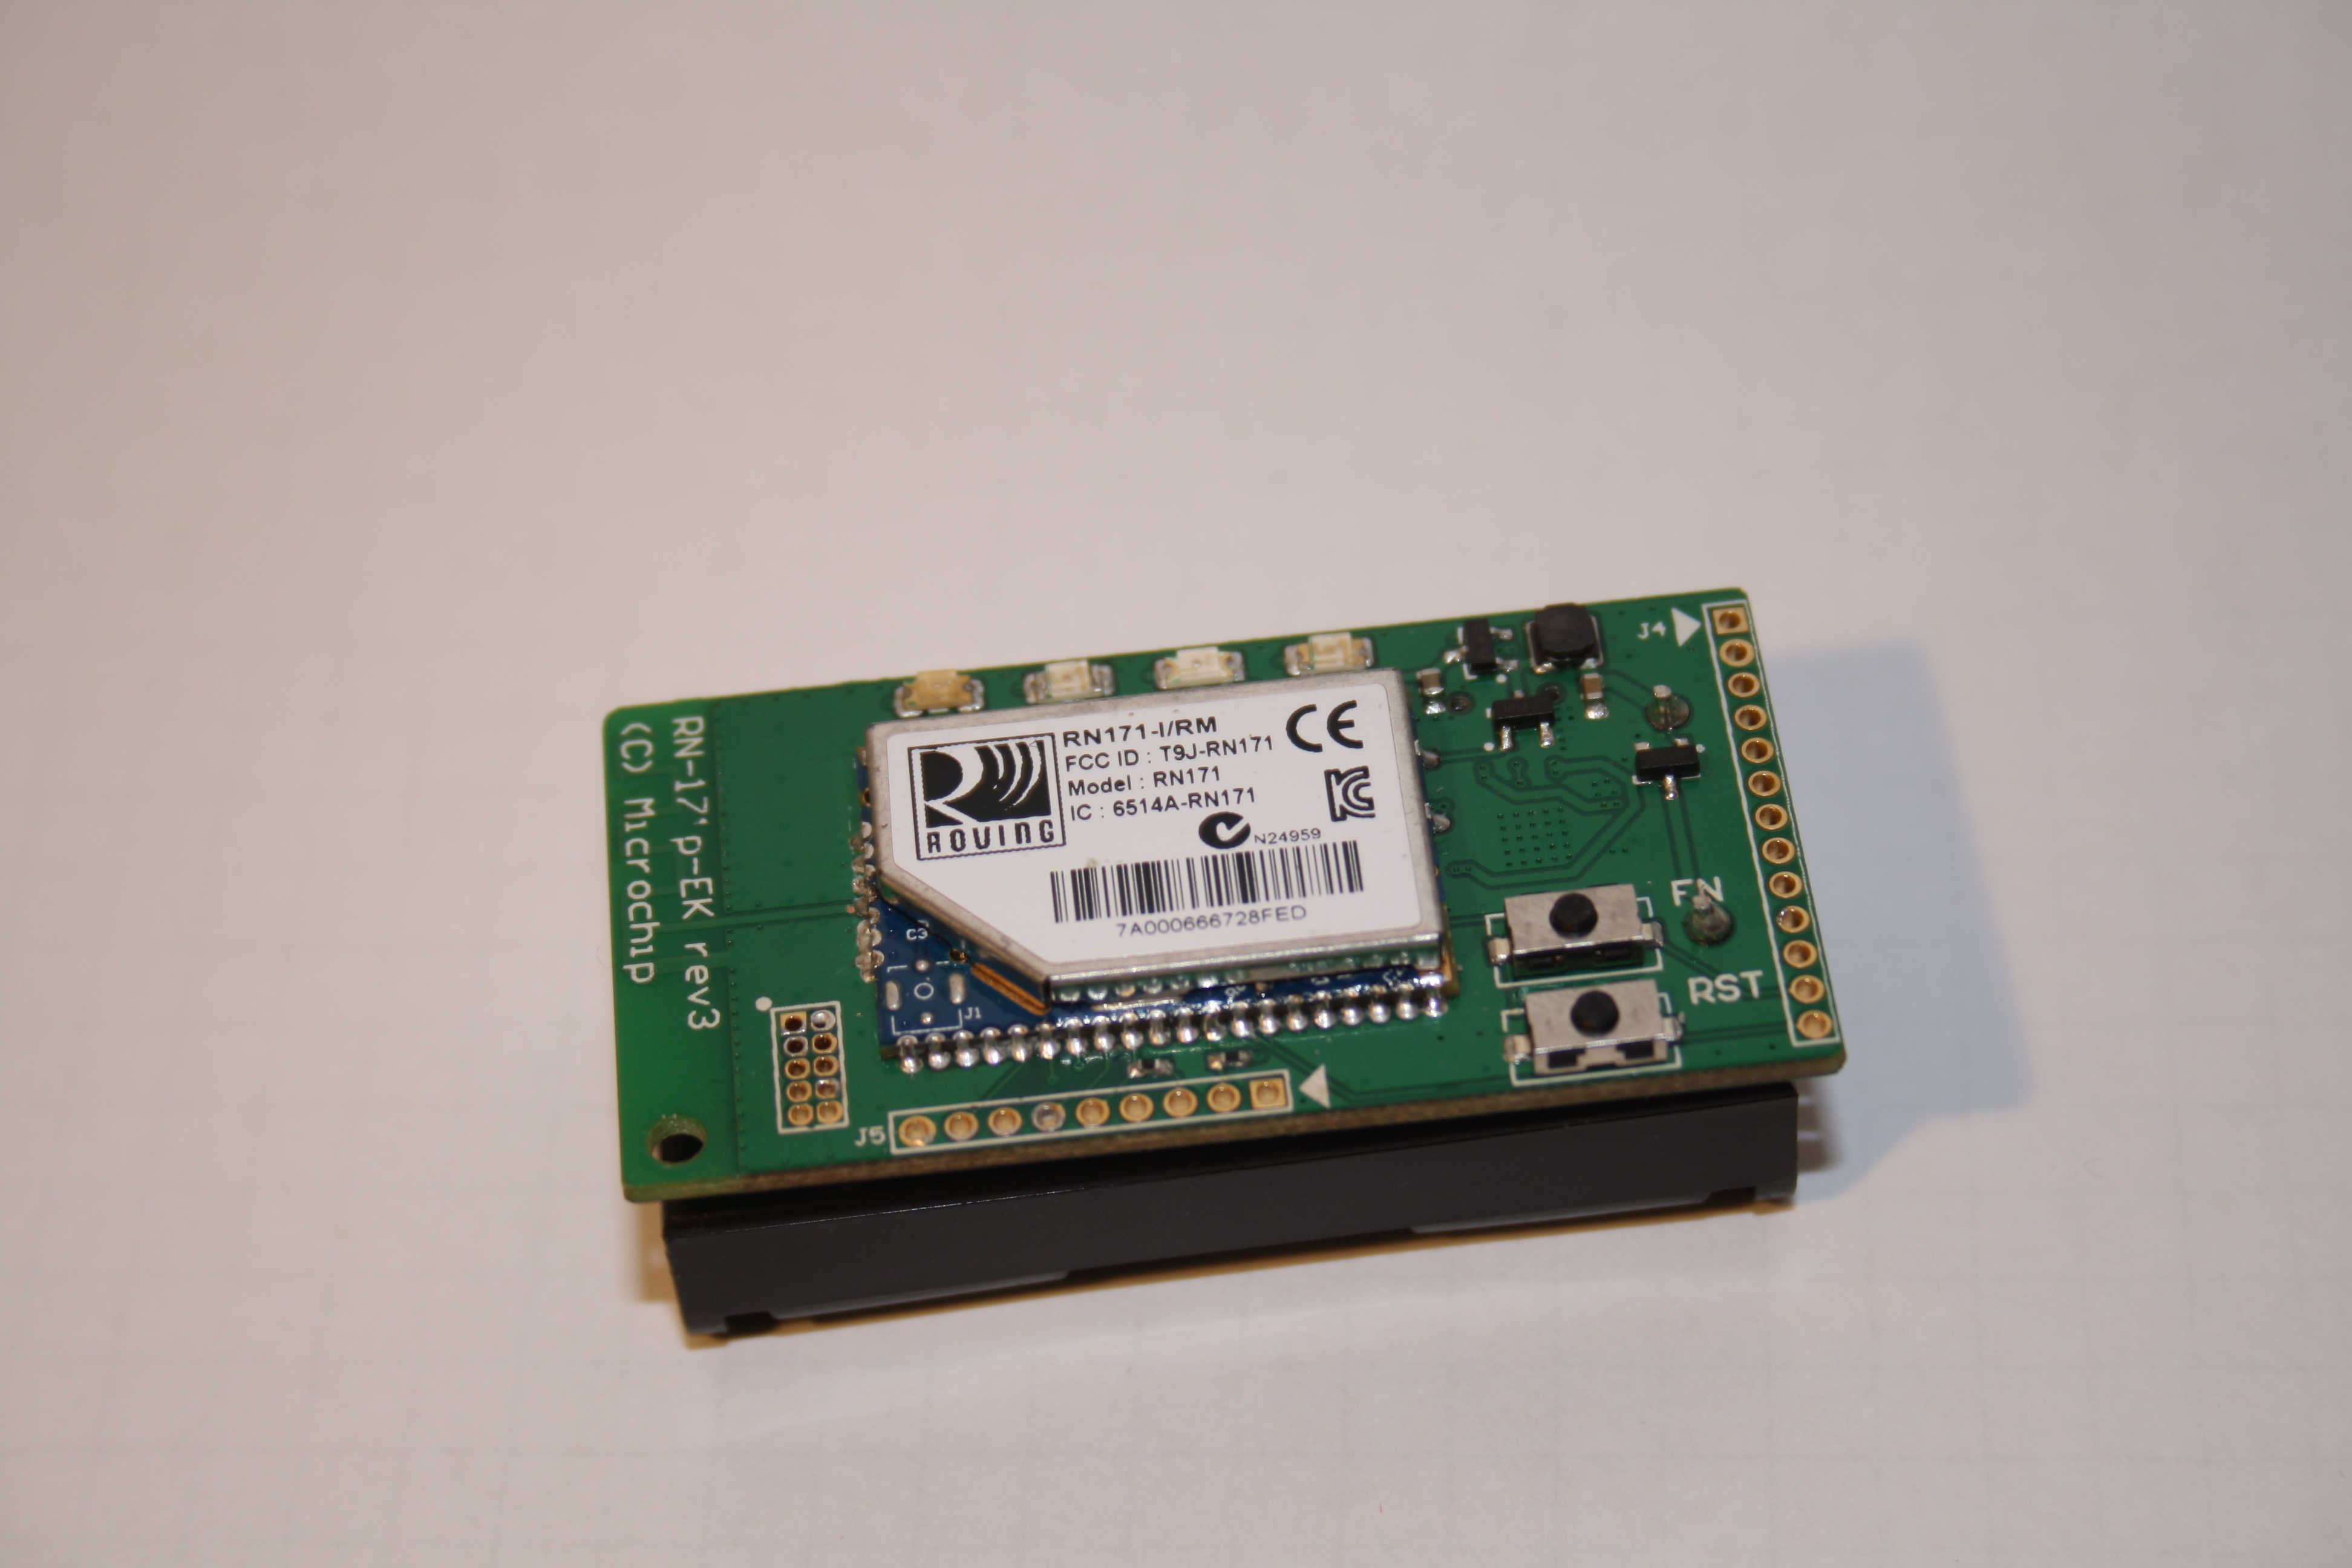
\includegraphics[width = 0.6\textwidth]{Bilder/RN171_EK}
    \par\end{centering}
    \caption[RN171 Evaluation-Kit]{RN171 Evaluation-Kit\cite{RN171_EK_source}}
    \label{RN171_EK}
  \end{figure}

  Um das WLAN-Modul so einzustellen, dass es sich Pin-gesteuert mit einem Host verbindet sind einige Schritte notwendig:
  \begin{itemize}
    \item \textbf{\$\$\$}\\
    Öffnet den Commandmode, nun können die Einstellungen vorgenommen werden
    \item \textbf{set wlan ssid <network\_name>}\\
    Deklariert den Netzwerknamen
    \item \textbf{set wlan phrase <network\_passphrase>}\\
    Deklariert das Passwort mit dem das Netzwerk gesichert ist
    \item \textbf{set ip host <host\_ip-address>}\\
    Deklariert die IP-Adresse des Empfängers
    \item \textbf{set ip remote <host\_portnumber>}\\
    Deklariert den Port auf dem der Empfänger die Daten empfangen soll
    \item \textbf{set sys iofunc 0x70}\\
    Durch diese Einstellung kann das WLAN-Modul über die Pins gesteuert werden
    \item \textbf{set wlan join 1}\\
    Stellt das WLAN-Modul auf automatisches Verbinden mit dem angegebenen Netzwerk ein
    \item \textbf{set ip protocol 4}\\
    Stellt das WLAN-Modul auf eine TCP/IP-Verbindung ein bei der nur Daten vom gespeicherten Host akzeptiert werden
    \item \textbf{set uart baud <desired-baudrate>}\\
    Stellt die Baudrate des WLAN-Moduls ein, Standard ist 9600
    \item \textbf{save}\\
    Speichert die Parameter in den Standardeinstellungen die nach einem Neustart geladen werden
    \item \textbf{reboot}\\
    Erzeugt einen Neustart bei dem die Standardeinstellungen geladen werden
  \end{itemize}
  Nachdem das WLAN-Modul auf die nötigen Parameter eingestellt ist, kann es direkt mit dem Mirkocontroller verbunden werden, die Verbidnung kann über einzelne Pins kontrolliert
  werden.

  \subsection{Herausforderungen und Lösungen}
  Eine Herausforderung stellte die Frage dar wie genau die Verbindung hergstellt wird. Das Datenblatt des WLAN-Moduls mit über 100 Seiten bietet viele potentielle Möglichkeiten.
  Die erste Wahl fiel auf das Auslesen einer Website, auf den ersten Anblick funktionierte das auch, jedoch musste festgestellt werden, dass unabhängig von der Website sehr ähnliche
  Daten verarbeitet werden, jedoch nicht der eigentliche Inhalt der Website sondern Providerinformationen.

  Die zweite Wahl fiel auf eine TCP/IP Verbindung, lediglich die genaue Umsetzung dieser ließ viele Möglichkeiten offen. Einerseits besteht die Möglichkeit eine Verbindung direkt
  über die Eingabe "open" im Commandmode zu öffnen, andererseits jedoch auch über die Pins als auch automatische Timeouts.

  Aufgrund der Einfachheit und vollen Kontrolle viel die Wahl auf die Ansteuerung über die Pins.
  Dazu stehen 3 unterschiedliche Pins zur Verfügung:
  \begin{itemize}
    \item \textbf{Associated}\\
    Mit einem Netzwerk verbunden
    \item \textbf{Open TCP connection}\\
    Die Verbidnung zum Host herstellen
    \item \textbf{Connected}\\
    Die Verbindung zum Host ist hergestellt
  \end{itemize}
  Die Statusinformationen Associated als auch Connected werden von dem WLAN-Modul geliefert, die Anweisung eine Verbindung herzustellen von dem Mirkocontroller.

%%%%%%%%%%%%%%%%%%%%%%%%%%%%%%%%%%%%%%%%%%%%%%%%%%%%%%%%%%%%%%%%%%%%%%%%%%%%%%%
\section{Schnittstelle Applikation}


  \subsection{Technische Planung}

  \subsection{Umsetzung}

  \subsection{Herausforderungen und Lösungen}


% !TEX root = diplomarbeit.tex
\chapter{Mechanik}

\renewcommand{\kapitelautor}{Autor: Alexander Punz}

\section{Allgemeine technische Planung}

		\subsubsection{Allgemeine Informationen über 3D Drucken}

		Die Technologie des 3D Druckens hat in den letzten Jahren immer mehr an Popularität gewonnen. Mit Hilfe des 3D Druckers kann man fast alle vorstellbaren Formen anfertigen.
		Es gibt verschiedenste Verfahren wie man ein Werkstück anfertigen kann: Laser Sintern, Stereolithographie, Drucken mit flüssigen Materialien, etc.
		In diesem Projekt wird nur die Variante des Druckens mit flüssigen Material verwendet.
		Diese ist kostengünstig \bzw genau genug für die Teile. Wie der Name schon sagt, wird Material in einem Druckkopf geschmolzen und dann Schicht für Schicht auf der Druckplatte aufgetragen.
		Der Druckkopf fährt nur in X und Y Richtung, die Höhe wird mit der Druckplatte selbst verfahren.

		Meist werden Drucker über einen Maschinencode gesteuert, dem sogenannten „G-Code“. In diesem Code werden die Punkte (Koordinaten) definiert, die der Extruder (Druckkopf) abfahren muss.
		Die folgende Abbildung zeigt ein Beispiel eines Maschinencodes.

			\begin{figure}[tbh]
			\begin{centering}
			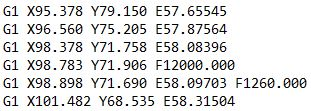
\includegraphics[width = 0.45\textwidth]{Bilder/gcode_erklaerung}
			\par\end{centering}
			\caption{Maschinencode Erklärung}
			\label{gcode_erklaerung}
			\end{figure}

			% Table generated by Excel2LaTeX from sheet 'Tabelle1'
			\begin{table}[htbp]
  		\centering
  		\caption{Befehle G Code}
	    \begin{tabular}{ll}
	    G1    & Kontrollierte Bewegung \\
	    X, Y  & Koordinaten in horizontaler und vertikaler Richtung \\
	    E     & Angabe der Menge des Filaments, dass in den Extruder geschoben werden muss \\
	    F     & Geschwindigkeit, mit der das Material in den Extruder geschoben wird (mm/min) \\
	    \end{tabular}%
	  	\label{tab:befehle gcode}%
			\end{table}%

		Je nachdem wie der Drucker aufgebaut ist, werden die Produkte genau oder nur grob angefertigt. Sehr genaue Teile kann man am besten in einem Drucker produzieren, der einen geschlossenen Druckraum \bzw eine beheizte Druckplatte hat.
		Besonders an dünnen Platten merkt man das. Wenn der Druckraum nach \bzw während des Druckvorgangs warm ist, kühlt das Werkstück an jeder Stelle fast gleich ab.
		Ist der Druckraum offen, kühlt das Werkstück in der Mitte schneller ab, kühles Material zieht sich zusammen, daher biegt sich das Material auf.

		Es kann vorkommen, dass ein Teil nur so gedruckt werden kann, wenn es nicht komplett auf der Druckplatte aufliegt zum Beispiel ein Steg, der „in der Luft“ liegt oder eine Bohrung im Werkstück, die horizontal gedruckt werden muss.
		In solchen Fällen, druckt der Drucker unter diesem Steg Stützmaterial. Basierend auf diesem Stützmaterial, wird dann die gewünschte Form gedruckt.
		Das Stützmaterial ist so gefertigt, dass man es leicht von dieser abbrechen kann, ohne dass Rückstände zurück bleiben.

		\subsubsection{Materialeigenschaften}

		\subsubsection{Von der Idee zur Anfertigung}

		Die größte Hürde an der Realisierung einer Idee ist, eine CAD Zeichnung zu erstellen. In 3D CAD Programmen wie Creo, SolidWorks, etc. kann man ein Teil konstruieren und dann als STL (Standard Triangulation Language) File abspeichern.
		Dieses Format gibt dann nur mehr Informationen über die Oberfläche und Struktur an (siehe Abbildung \ref{stl_file_optionen}).
		Die Sehnenhöhe gibt an wie genau die Oberfläche gedruckt werden muss, die Winkelsteuerung gibt die Genauigkeit der Radien und Kanten des Teiles an.


			\begin{figure}[tbh]
			\begin{centering}
			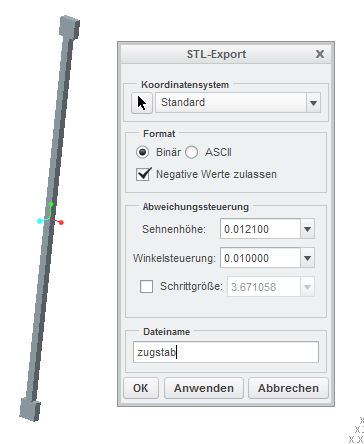
\includegraphics[width = 0.5\textwidth]{Bilder/stl_file_optionen}
			\par\end{centering}
	 		\caption{Einstellung für STL File}
			\label{stl_file_optionen}
			\end{figure}

		Mit diesem File kann man anschließend in Programmen wie Slic3r den gewünschten Maschinencode generieren lassen.
		In diesen Programmen gibt man die Lage des Werkstückes an \bzw in genaueren Einstellungen auch die Temperatur des Druckbettes, den Geschwindigkeiten und ähnliche Konfigurationen.

		Am häufigsten haben die Drucker eine USB Schnittstelle, \bzw verfügen über einen SD Karten Slot.
		Der Maschinencode wird auf diesen Speichermedien gespeichert und einfach auf den Drucker überspielt.

				\newpage


\section{Halterung für Cupcakes}

		\subsection{Technische Planung}

		Die Diplomarbeit hat sich speziell auf den Transport von Cupcakes spezialisiert, um diesen sicher transportieren zu können, ist es notwendig eine Halterung zu konzipieren.
		Zu beachten ist, dass die Halterung möglichst wenig wiegt \bzw leicht zu montieren ist.

		Der Akku wurde an der Unterseite des Hexacopters befestigt, daher war es nur mehr möglich die Halterung an der oberen Centerplate zu platzieren.
		Damit der Multicopter möglichst ausgewogen ist, muss sich das zu transportierende Objekt in der Mitte befinden.
		Die Idee war es daher, den Cupcake mit einer Halterung zu umranden, um ihn gegen Verrutsche zu sichern. Die Geometrie der Platte \bzw die Größe des Objektes hat die Befestigungsmöglichkeiten etwas eingeschränkt (siehe Abbildung \ref{platte_cupcake}).
		Die innere Reihe der Langlöcher würde sich optimal anbieten, um die Halterung befestigen zu können, die Cupcakeform kann so direkt von einer Haltevorrichtung gestützt werden.


			\begin{figure}[tbh]
			\begin{centering}
			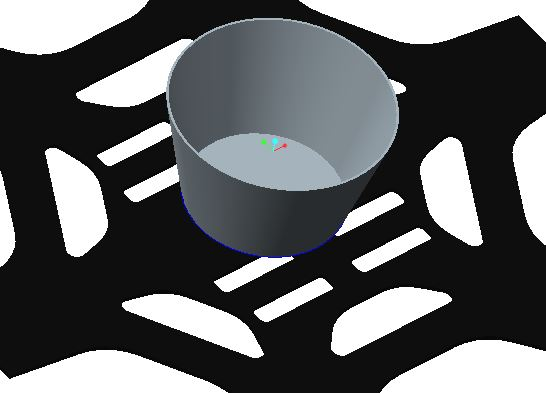
\includegraphics[width = 0.5\textwidth]{Bilder/platte_cupcake}
			\par\end{centering}
			\caption{Position Cupcake}
			\label{platte_cupcake}
			\end{figure}

	\subsection{Umsetzung}

	Wie schon in der technischen Planung erwähnt wurde, sollte der Cupcake von einer Haltevorrichtung umrandet werden.
	Die inneren Ausnehmungen der oberen Centerplate haben sich optimal angeboten, da diese direkt bis zur Form reichen.

	Es wurden Stützen konstruiert, die in den Ausnehmungen fixiert werden können und sich direkt an das Dessert anpassen.
	Die folgenden Abbildungen zeigen die konstruierten Halterungsstutzen und deren Befestigung.

			\begin{figure}[H]
			  \begin{centering}
			    \subfigure[Halterung Cupcake oben\label{halterung_cupcake_oben_grosz}]{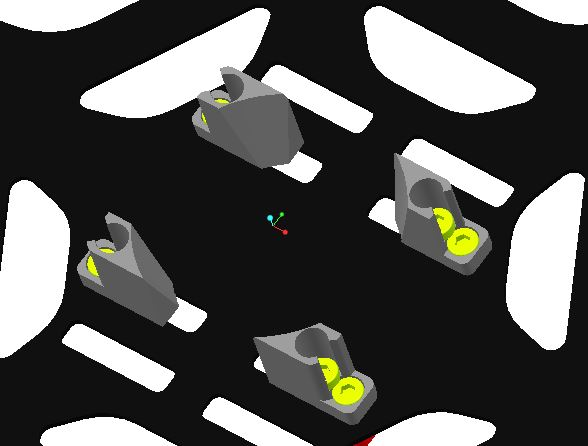
\includegraphics[width = 0.4\textwidth]{Bilder/halterung_cupcake_oben_grosz}}
			    \subfigure[Halterung Cupcake unten\label{halterung_cupcake_unten_grosz}]{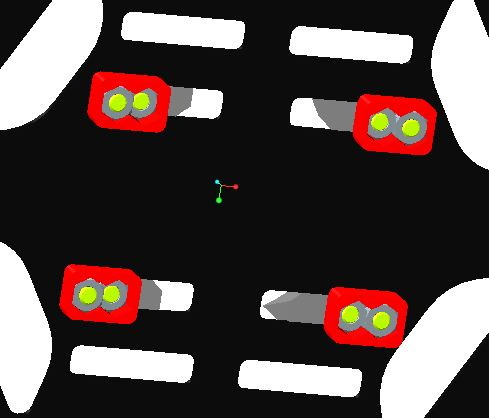
\includegraphics[width = 0.4\textwidth]{Bilder/halterung_cupcake_unten_grosz}}
			  \par\end{centering}
			  \caption{Halterung Cupcake}
			  \label{Halterung_Cupcake}
			\end{figure}

	Die Stützen (siehe Abbildung \ref{halterung_cupcake_oben_grosz}) wurden so entworfen, dass sie sich dem Radius \bzw der Höhe der Form des Cupcake anpassen.
	Die Höhe der Halterung wurde so gewählt, dass etwa die Hälfte der Cupcakeform frei liegt.
	Das soll vermeiden, dass man sich die Finger beim Entnehmen des Cupcakes an der Creme schmutzig macht.

	Die Halterung wird direkt an der Centerplate mit Durchgangsschrauben und Muttern festgeschraubt.
	Durch den Platzmangel mussten M4 Schrauben gewählt werden, da diese klein sind und trotzdem viel Beanspruchung aufnehmen können.
	Die Schlüsselweite einer M4 Mutter beträgt 7.0 mm, die Breite der Ausnehmung 6.5 mm, würde man die Schrauben direkt mit der Platte verschrauben, müsste man eine Beilagscheibe zwischenlegen, um eine größere Aufliegefläche für die Mutter zu erhalten.

	Es wurden spezielle Mutterhalter entworfen (siehe Abbildung \ref{halterung_cupcake_unten_grosz}), diese bezwecken zwei Funktionen:
	Einerseits muss man die Muttern während man die Halterung montiert nicht mehr festhalten und andererseits kann man die Schraubenverbindung viel fester anziehen, da man die Platte nicht mehr beschädigen kann.

	Der Platz für die Stutzen entlang der Langlöcher ist nur so kurz, dass sich die Köpfe der Schrauben und die Muttern schneiden würden.
	Um dieses Problem zu beheben, wurden Höhenunterschiede zwischen den Schrauben eingeplant.
	Das macht die Halterungsstutzen kompakter und verhindert Kollisionen.

	\subsection{Herausforderungen und Lösungen}

	Die größte Herausforderung beim Konstruieren war es, die Halterung an die Form des Cupcakes anzupassen.
	Die Halterungsstützen sollen an die Rundung \bzw den Durchmesserverlauf der Cupcakeform angepasst werden.
	Um die richtige Form der Stützen konstruieren zu können, wurde erst der Winkel der Cupcakeform mit der  folgenden Formel ermittelt:

			\begin{figure}[H]
			\begin{centering}
			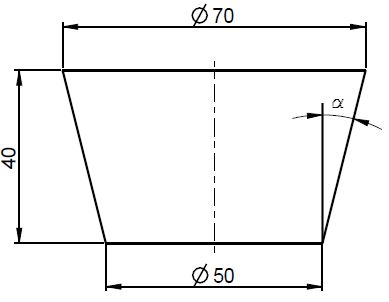
\includegraphics[width = 0.4\textwidth]{Bilder/berechnung_winkel}
			\par\end{centering}
			\caption{Berechnung des Winkels}
			\label{berechnung_winkel}
			\end{figure}

			\[
 				\tan \alpha = \frac{35mm-25mm}{40mm}  \qquad \alpha = \arctan \frac{35mm-25mm}{40mm} = \SI{14.04}{\degree}
 			\]

	Konstruiert wurde die Halterung mit einem Winkel von 15° um Ungenauigkeiten des Druckers besser kompensieren zu können.

	In der folgenden Abbildung kann man erkennen, dass manche Wände bei den Bohrungen zu dünn sind zu drucken, es entstehen dadurch Löcher.
	Dieses Problem könnte man nur lösen, wenn man die Schrauben weiter nach außen legen würde, jedoch ist das in diesem Fall nicht möglich, da die Ausnehmungen zu kurz sind.


			\begin{figure}[tbh]
			\begin{centering}
			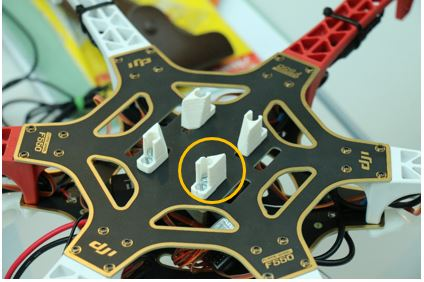
\includegraphics[width = 0.65\textwidth]{Bilder/halterung_cupcake_fertig_hinweis}
			\par\end{centering}
			\caption{Gedrucktes Halterungssystem}
			\label{halterung_cupcake_fertig_hinweis}
			\end{figure}

			\newpage

\section{Rotorschutz}

	\subsection{Technische Planung}

	In dem gewählten Bausatz des Hexacopters ist kein Rotorschutz vorhanden.
	Da der Hexacopter direkt zu den Gästen fliegen wird, ist es nicht umgänglich, den Kontakt mit den Propellern zu verhindern.
	Diese können durch die hohen Drehzahlen und die Kraft der Motoren erhebliche Verletzungen zuführen.
	Es gibt diverse Vorrichtungen für Multicopter zu kaufen, die nur die Rotorblätter schützen, jedoch keine, die auch das Eingreifen einer Hand verhindern.

	Der Rotor-, oder auch Propellerschutz genannt, soll wie ein Ring um die Rotorblätter liegen und auch auf der Ober,- und Unterseite Schutz vor Verletzungen bieten.
	Zu beachten ist jedoch auch, dass sechs Schutzvorrichtungen benötigt werden, daher sollten diese so leicht wie möglich sein, um das maximale Abfluggewicht nicht zu überschreiten.

	\subsection{Umsetzung}

	Die folgenden Abbildungen zeigen den konstruierten Propellerschutz, an dem Hexacopter montiert.

			\begin{figure}[tbh]
			\begin{centering}
			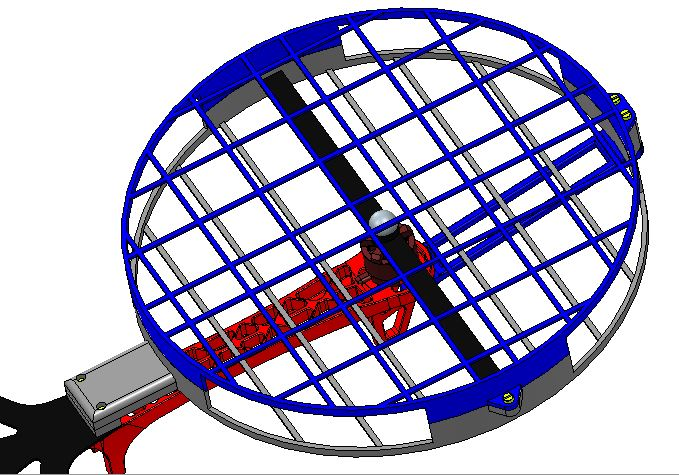
\includegraphics[width = 0.8\textwidth]{Bilder/propellerschutz_gesamt_oben}
			\par\end{centering}
			\caption{Propellerschutz oben}
			\label{propellerschutz_gesamt_oben}
			\end{figure}

			\begin{figure}[H]
			\begin{centering}
			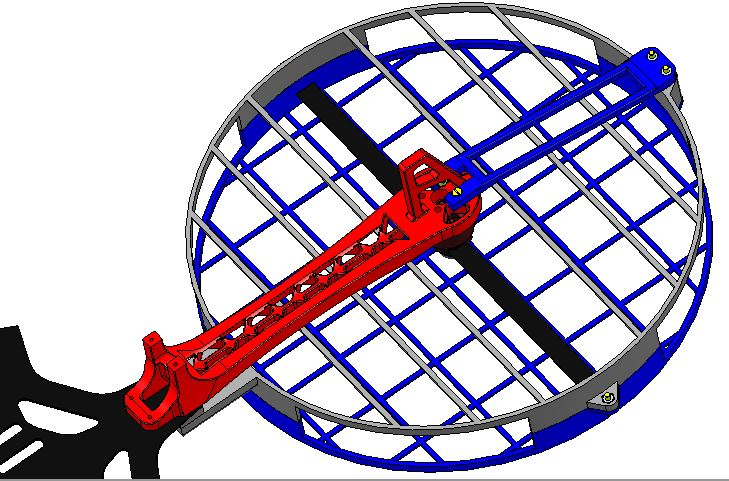
\includegraphics[width = 0.8\textwidth]{Bilder/propellerschutz_gesamt_unten}
			\par\end{centering}
			\caption{Propellerschutz unten}
			\label{propellerschutz_gesamt_unten}
			\end{figure}

	Wie geplant, umrandet der Ring das komplette Rotorblatt, im Falle eines Absturzes kann der Propeller nicht den Boden berühren und wird somit nicht beschädigt.
	Auf der Oberseite und Unterseite ist ein Gitter vorgesehen, welches Verletzungen an Personen verhindert.
	Das Gitter an der Oberseite ist etwas feiner gegliedert als an der Unterseite, da man den Cupcake von der oberen Centerplate entnehmen muss.
	An der Unterseite ist das Gitter nur gestreift konstruiert, da die Luftströmung nicht stark beeinflusst werden darf und die größere Verletzungsgefahr an der Oberseite besteht.

	Der komplette Rotorschutz wird einerseits mit zwei Schrauben am Hexacopter befestigt (siehe Abbildung \ref{propellerschutz_gesamt_oben}) und andererseits von einer Stütze (siehe Abbildung  \ref{propellerschutz_gesamt_unten},
	\textcolor{blue}{blauer Balken}) an der Unterseite gehalten. Die Stütze wird direkt an dem Motor angeschraubt, samt dem Arm des Hexacopters.
	Da die Schrauben der Centerplate und des Motors zu kurz sind, werden passende Zylinderkopfschrauben verwendet.
	Besonders bei dem Motor ist es wichtig, dass diese nicht zu lang sind, da sich der Motor nicht mehr bewegen könnte.

	Durch die Gewichtsbegrenzung \bzw der Form des Propellerschutzes, bot es sich an, diesen in einem 3D Drucker anzufertigen.
	Dazu wurde der Ring in zwei Hälften unterteilt, eine Ober,- und eine Unterseite.
	Der Ring hat einen ungefähren Innendurchmesser von 270 mm, das Druckbett eine maximale Abmessung von 270x210 mm.
	Beide Hälften mussten noch in weitere, für den Drucker passende Teile unterteilt werden.
	Die obere Hälfte wurde noch einmal in der Mitte geteilt, die Unterseite musste in vier Teile unterteilt werden (siehe folgende Abbildung \ref{propellerschutz_mitte_unterteilung}).

			\begin{figure}[tbh]
			\begin{centering}
			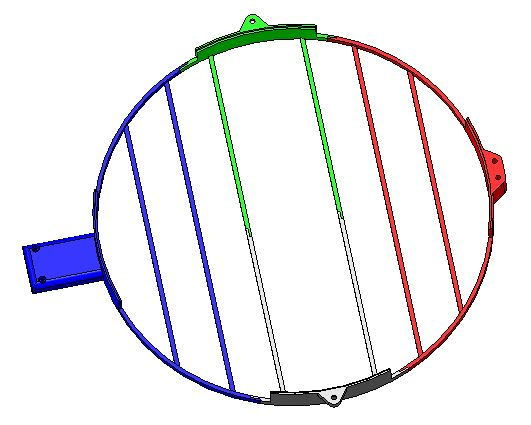
\includegraphics[width = 0.7\textwidth]{Bilder/propellerschutz_mitte_unterteilung}
			\par\end{centering}
			\caption{Propellerschutz Unterteilung}
			\label{propellerschutz_mitte_unterteilung}
			\end{figure}

			\begin{figure}[H]
			\begin{centering}
			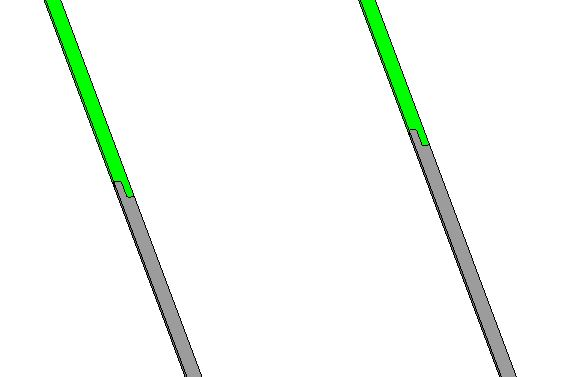
\includegraphics[width = 0.45\textwidth]{Bilder/propellerschutz_klebestellen}
			\par\end{centering}
			\caption{Propellerschutz Klebestellen}
			\label{propellerschutz_klebestellen}
			\end{figure}

	Die einzelnen Hälften  werden mit Sekundenkleber zusammengefügt, die Klebestellen wurden daher mit Nuten versehen,
	um eine größere Klebefläche zu gewährleisten (siehe Abbildung \ref{propellerschutz_klebestellen}).
	Die geklebten Hälften werden dann mit Durchgangsschrauben und Sechskantmutter miteinander verschraubt (siehe Abbildung  \ref{propellerschutz_mitte_unterteilung}),
	der kleine Absatz an der unteren Hälfte wird extra angefertigt da der Drucker kein Stützmaterial drucken müsste.

	\subsection{Herausforderungen und Lösungen}

	Eines der größten Probleme war es, den Rotorschutz so zu konstruieren, dass er stabil, aber auch sehr leicht ist.
	Im Falle eines Absturzes, würden hohe Kräfte auf den Propellerschutz wirken, daher muss dieser sehr robust gefertigt sein.
	Der Vorteil von ABS \bzw 3D Druckteilen ist, dass diese sehr elastisch sind, nicht wie Styropor zum Beispiel, es ist daher nicht notwendig den Ring dickwandig zu konstruieren.
 	Durch diesen Vorteil kann man einiges an Gewicht einsparen, das Problem besteht aber trotzdem noch darin, dass der Ring enorme Dimensionen hat.
	Eine komplette Zusammenstellung (Ring, Stütze und Schrauben) hat ein Gewicht von etwa 90 g.
	Auf sechs Propeller aufgerechnet mehr als ein halbes Kilogramm, der Hexacopter kann das zwar noch tragen, jedoch schränkt das die hardwaremäßige Erweiterung stark ein.

	Eine weitere Herausforderung war es, den Ring anzufertigen. Wie schon in dem oberen Punkt erklärt wurde, musste der Ring in sieben Teile unterteilt werden.
	Die Herausforderung lag darin, die Stücke so zu gliedern, damit sie im 3D Drucker fertigbar sind und nicht zu viel Druckzeit auf sich nehmen.
	Die Druckzeit wurde zwar schon optimiert durch die Gliederung, jedoch braucht es trotzdem noch etwa 14 Stunden alle Teile für einen Rotorschutz zu drucken.

	\subsection{Implementierung}

Die einzelnen Teile wurden wie schon erwähnt, miteinander verklebt. Bevor diese zusammengefügt wurden, musste sichergestellt werden, dass die Nuten exakt ineinander passen.
Würde dies nicht gewährleistet sein, würden die obere und untere Hälfte des Propellerschutzes nicht mehr zusammenpassen.
Die Toleranzen des Druckers, besonders bei solchen Stellen sind so groß, dass man meistens mit Feilen die Nuten nachbessern muss.
Besonders beim Verkleben der Teile ist viel Geduld nötig, da auch der Sekundenkleber nicht sofort komplett trocken ist,
es war ebenso wichtig, den richtigen Untergrund zu wählen, eine Holzplatte eignete sich am besten, da keine Rückstände blieben.

Die beiden Hälften wurden dann miteinander verschraubt, samt der Stütze.
Der gesamte Rotorschutz konnte dann mittels den vorgesehenen Schrauben an der Centerplate und dem Arm des Hexacopters befestigt werden.

			\newpage

\section{Halterung Ultraschallsensor}

	\subsection{Technische Planung}

	Die Höhe des Hexacopters wird mittels eines Ultraschallsensors gesteuert, dieser misst den Abstand von dem Boden aus.
	Damit der Sensor genaue Werte messen kann, muss er fest auf dem Multicopter befestigt werden.
	Um das gewährleisten zu können, musste eine Halterung entworfen werden, die den Ultraschallsensor optimal mit dem Hexacopter verbindet.
	Die Anforderungen an die Halterung begrenzen sich auf ein geringes Gewicht \bzw eine einfache Montagemöglichkeit.
	Der Sensor hat auf jeder Ecke eine kleine Bohrung von 1.5 mm vorgesehen, das erschwert die Befestigungsmöglichkeit des Sensors an der Halterung, da es keine gängigen Schrauben in dieser Größe gibt.

	\subsection{Umsetzung}

	Die folgende Abbildung (Abbildung \ref{halterung_ultraschall}) zeigt die CAD Konstruktion und die gefertigte (Abbildung \ref{halterung_ultraschall_fertig}) Ultraschallsensorhalterung.

			\begin{figure}[H]
				\begin{centering}
					\subfigure[CAD Konstruktion Ultraschallsensorhalterung\label{halterung_ultraschall}]{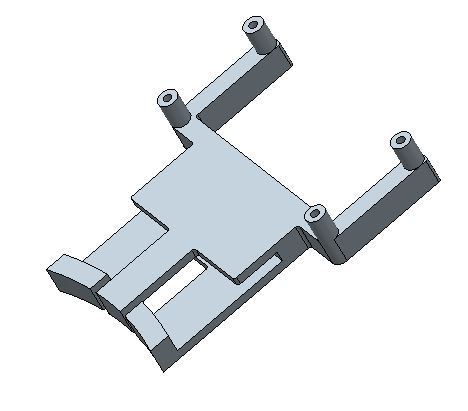
\includegraphics[width = 0.4\textwidth]{Bilder/halterung_ultraschall}}
					\subfigure[Gefertigte Ultraschallsensorhalterung\label{halterung_ultraschall_fertig}]{\includegraphics[width = 0.4\textwidth]{Bilder/halterung_ultraschall_fertig}}
				\par\end{centering}
				\caption{Ultraschallsensorhalterung}
				\label{Halterung_Ultraschallsensor}
			\end{figure}

	Das Gewicht spielte, analog zu den anderen Konstruktionen, eine wichtige Rolle.
	Materialien wie Stahl oder Aluminium wären selbst bei diesem kleinen Teil (51x46x10 mm) zu schwer geworden.
	Um das zu verhindern wurde diese Haltevorrichtung, wie auch der Propellerschutz, in einem 3D Drucker angefertigt.
	Das Teil wiegt durch die Fertigungsmethode etwa 5.5 g, das entspricht etwa dem Gewicht einer 20 Cent Münze.

	Die Halterung wird an der unteren Centerplate befestigt, da wie schon erwähnt, der Sensor von dem Boden aus misst.
	Die Befestigungsmethode ist selbst entwickelt worden, dabei handelt es sich um ein spezielles Klammersystem, welches an einer Strebe der Platte montiert werden kann (siehe Abbildung \ref{halterung_ultraschall_fertig}).
	Die Klammer besteht aus drei Stegen, auf denen jeweils ein Anschlag vorgesehen wurde.
	Die Form der Anschläge ist  exakt an die Centerplate angepasst, damit sich die Halterung so geringfügig wie möglich bewegen lässt.

	Die ideale Stärke der Stege wurde durch Versuche ermittelt, es wurde dabei das Klammersystem mit unterschiedlichen Dicken gefertigt und an dem Hexacopter getestet.
	Die optimale Stärke war deshalb wichtig, da das System nicht funktionieren würde, wenn diese falsch dimensioniert werden würde.
	Die Elastizität des Materials \bzw die gewählte Dicke der Stege ermöglicht es, diese soweit auseinanderziehen zu lassen, dass die Anschläge einfach über die Platte geschoben werden können.
	Aufgrund dieser Eigenschaften verformen sich diese auch wieder komplett zurück und fixieren somit die Halterung.

	Damit der Sensor nicht nach unten kippen kann, wurde eine Nut in die Haltevorrichtung vorgesehen.
	Droht die Halterung nach unten zu kippen, verkeilt sich diese mit der Centerplate und kann nicht mehr weitersinken.
	Die Nut ist so groß dimensioniert worden, dass sie leicht auf die Platte geschoben werden aber sich nur minimal bewegen lässt.

	Der zweite Teil der Halterung wurde so konstruiert, dass die vier Ecken der Sensorplatine gleichmäßig aufliegen können.
	Auf dem Ultraschallsensor selbst befinden sich jedoch vier Anschlussstifte, die es nicht ermöglichen, die Platine direkt auf der „Gabel“ zu befestigen.
	Um Kabel trotzdem problemlos anschließen zu können, wurde der Sensor mittels vier Stutzen 5 mm höher gelegt.

	Geplant wurde, dass der Sensor an den Stutzen mit vier Blechschrauben befestigt wird, die Durchmesser der Bohrungen sind aber so klein, dass keine gängigen Schraubendurchmesser verwendet werden können.
	Die geeigneten Schrauben werden nur in ausgewählten Geschäften verkauft, um einen viel höheren Preis \bzw längeren Lieferzeiten, als bei normalen Schrauben.
	Um den Sensor trotzdem befestigen zu können, wurden Kupferdrähte zur Fixierung verwendet.
	Da nur das Gewicht des Ultraschallsensors an den Drähten zieht, geben diese selbst bei heftigen Flugmanövern nur minimal nach.

	\subsection{Herausforderungen und Lösungen}

	Das Klammersystem hat die meiste Zeit auf sich genommen.
	Die erste Version der Halterung hat gezeigt, dass die angenommenen Dimensionen nicht umgesetzt werden konnten.
	Das Problem lag darin, dass die Halterung nicht hochkant, sondern vertikal gedruckt werden musste.
	Damit die Haltevorrichtung gedruckt werden kann, hat der Drucker Stützmaterial in die Nut gedruckt.
	Dieses Stützmaterial kann jedoch nicht restlos entfernt werden, daher musste die Höhe des Spaltes vergrößert werden.
	Es brauchte drei verschiedene Versionen der Ultraschallsensorhalterung, bis alle Parameter ideal gepasst haben, das kostete natürlich Zeit, da jedes Mal ein neues Teil gedruckt werden musste.

	\subsection{Berechnungen}

	Die Halterung des Ultraschallsensor wurde so dimensioniert, dass der Ultraschallsensor \bzw im Falle eines Absturzes auch noch die auftretenden Kräfte getragen werden können,
	es ist trotzdem wichtig zu wissen, wie viel die Halterung maximal tragen kann.
	Sollte sich herausstellen, dass das Werkstück nicht richtig konstruiert wurde, muss man Maßnahmen treffen um die Belastbarkeit zu steigern.

	Man kann diese Belastungen händisch rechnen, jedoch ist das in diesem Fall sehr aufwändig, da die Lagerung sehr komplex zu rechnen wäre.
	Es ist einfacher die Beanspruchungen in Programmen wie Creo simulieren und auswerten zu lassen.
	Die Ergebnisse der Simulation sind so genau, dass man heutzutage in der Industrie nur mehr sehr selten solche Arten von Analysen händisch vornimmt.

	Die maximalen Belastbarkeiten sind für jeden Kunststoff anders, jede Firma verwendet andere Stoffe um bessere Leistungen erzielen zu können, je nach dem Anwendungsgebiet.
	Wollte man die Berechnungen auf die Kommastelle genau vornehmen, müsste man einen Zug,- oder Biegeversuch für den jeweiligen Werkstoff machen,
	um die tatsächlichen Eigenschaften zu ermitteln.

	In diesen Versuchen wird meist ein Stab mit einer vordefinierten Fläche und Länge hergestellt und dann in eine Zugprüfmaschine eingespannt.
	Die Zugprüfmaschine zieht den Stab langsam auseinander bis dieser reißt, diese bestimmte Kraft und die Fläche des Stabes ergeben die maximale Streckspannung.
	Diesen Versuch kann man analog dazu für die Biegung und Torsion machen, man erhält dadurch die maximale Bruch,- \bzw Torsionsspannung.

	Da sich die Werte der einzelnen Hersteller nur minimal voneinander unterscheiden,
	wurden in diesem Fall die Daten aus einer Tabelle eines anderen Kunstoffherstellers genommen (siehe Abbildung \ref{werte_abs}).

			\begin{figure}[H]
			\begin{centering}
			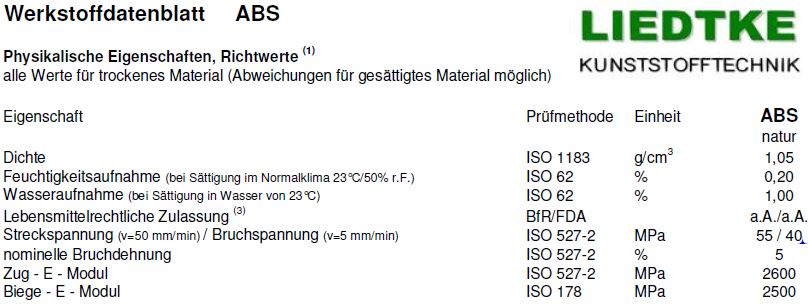
\includegraphics[width = 0.5\textwidth]{Bilder/werte_abs}
			\par\end{centering}
			\caption[Werte ABS]{Werte für ABS\cite{werte_abs}}
			\label{werte_abs}
			\end{figure}

	Wichtig sind die Angaben: Dichte, Streck,- und Bruchspannung, nominelle Bruchdehnung und Elastizitätsmodul für Zug/Biegung (E-Modul) des Materials.
	Diese Werte definieren die Eigenschaften des Materials, daher sind sie essenziell für die Berechnungen in Creo.

	Creo bietet mit seinen Funktionen exakte Analysen an, die die maximalen Belastbarkeiten so genau berechnen wie sie tatsächlich auftreten.
	In diesem Fall wurde die prinzipielle Situation simuliert, die Werte stimmen nicht exakt mit den realen Kräften überein, jedoch reichen diese um zu sehen, was passiert.

	In Creo steht eine große Auswahl an Einspannmöglichkeiten bis zu Belastungen für ein Werkstück zu Verfügung (siehe folgende Abbildung).

			\begin{figure}[H]
			\begin{centering}
			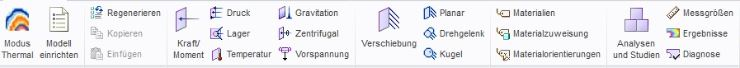
\includegraphics[width = 0.45\textwidth]{Bilder/auswahl_creo}
			\par\end{centering}
			\caption{Auswahlmenü Simulation}
			\label{auswahl_creo}
			\end{figure}

	Unter dem Menü „Verschiebung“ wird die gewünschte Lagerung definiert, man kann eine Fläche, Punkt oder Kante auswählen,
	je nachdem wie das Prüfwerkstück gelagert werden soll und in welche Richtung dieses verschiebbar ist.
	In dem Menü „Kraft/Moment“ gibt man dann an welche Belastung, in welcher Fläche/Punkt/Kante auf das Werkstück wirkt. Der Auswahlpunkt „Analysen und Studien“ startet die Simulation.

	Der Sensor wird so montiert, dass er die Halterung nach unten zieht, die Folge ist, dass sich die Halterung, grob angenommen,
	sich mit zwei Kanten an der Platte verkeilt (siehe Abbildung \ref{lager_darstellung_1} und \ref{lager_darstellung_2}).
	Die Lagerung wird daher so definiert, dass diese zwei Kanten als Festlager angenommen werden (in keine Richtung verschiebbar).

			\begin{figure}[H]
				\begin{centering}
					\subfigure[Lagerung 1. Stelle\label{lager_darstellung_1}]{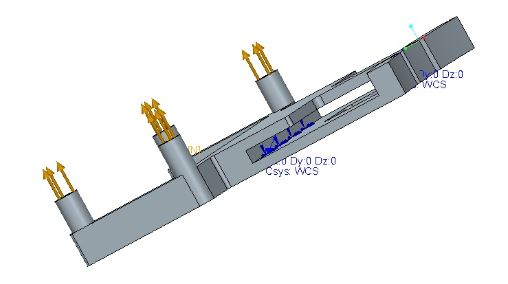
\includegraphics[width = 0.4\textwidth]{Bilder/lager_darstellung_1}}
					\subfigure[Lagerung 2. Stelle\label{lager_darstellung_2}]{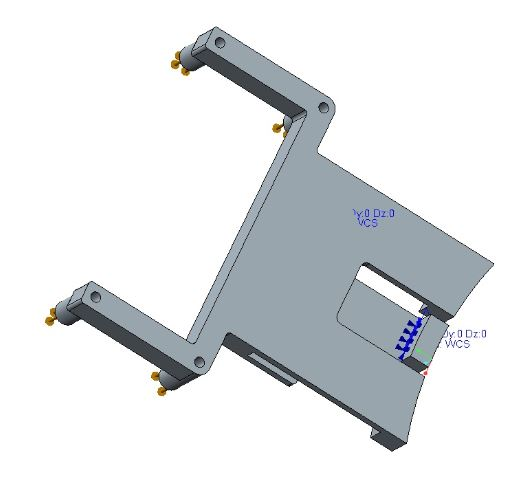
\includegraphics[width = 0.4\textwidth]{Bilder/lager_darstellung_2}}
				\par\end{centering}
				\caption{Lagerung der Halterung in Simulation}
				\label{Lagerung_Halterung}
			\end{figure}

	Der Ultraschallsensor wird durch eine Kraft ersetzt, diese kann man variieren, je nachdem um wieviel die Halterung belastet werden soll.
	Nachdem alle Parameter definiert wurden, konnte die Simulation gestartet werden.

	Es wurden zwei Simulationen durchgeführt, in der ersten wurde nur der Ultraschallsensor (8.5 g) als Belastung angenommen und im zweiten Fall  wurde die Halterung mit einer Last von 2 kg beansprucht.

	Die Abbildung \ref{max_spannung_f0_1_r0_5} zeigt das Ergebnis der ersten Simulation mit einer Kraft von 0.1 N (0,01 g).

			\begin{figure}[H]
			\begin{centering}
			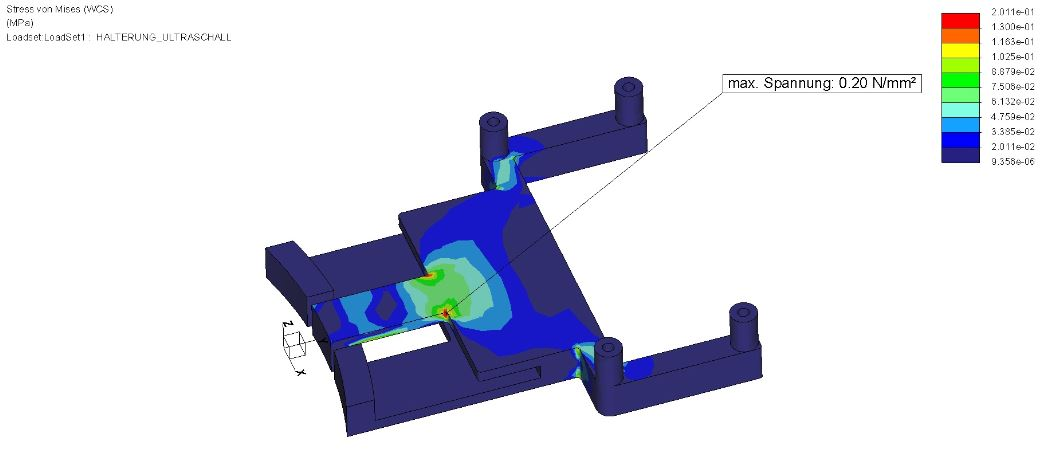
\includegraphics[width = 0.45\textwidth]{Bilder/max_spannung_f0_1_r0_5}
			\par\end{centering}
			\caption{max. Spannung bei 0.1 N}
			\label{max_spannung_f0_1_r0_5}
			\end{figure}

	Die maximale Spannung beträgt in diesem Fall etwa 0.20 N/mm^{2} an der oberen Lasche.
	Es ist zu sehen, dass diese Belastung die Halterung kaum beeinflusst, das bedeutet die angenommen Dimensionen reichen aus um den Sensor zu halten.

	Die Abbildungen \ref{max_spannung_f20_r0_5} und \ref{max_spannung_f20_r0_5_oben}  zeigen die Simulationsergebnisse mit einer Beanspruchung von 20 N (2 kg).

				\begin{figure}[H]
					\begin{centering}
						\subfigure[max. Spannung bei 20 N oben\label{max_spannung_f20_r0_5}]{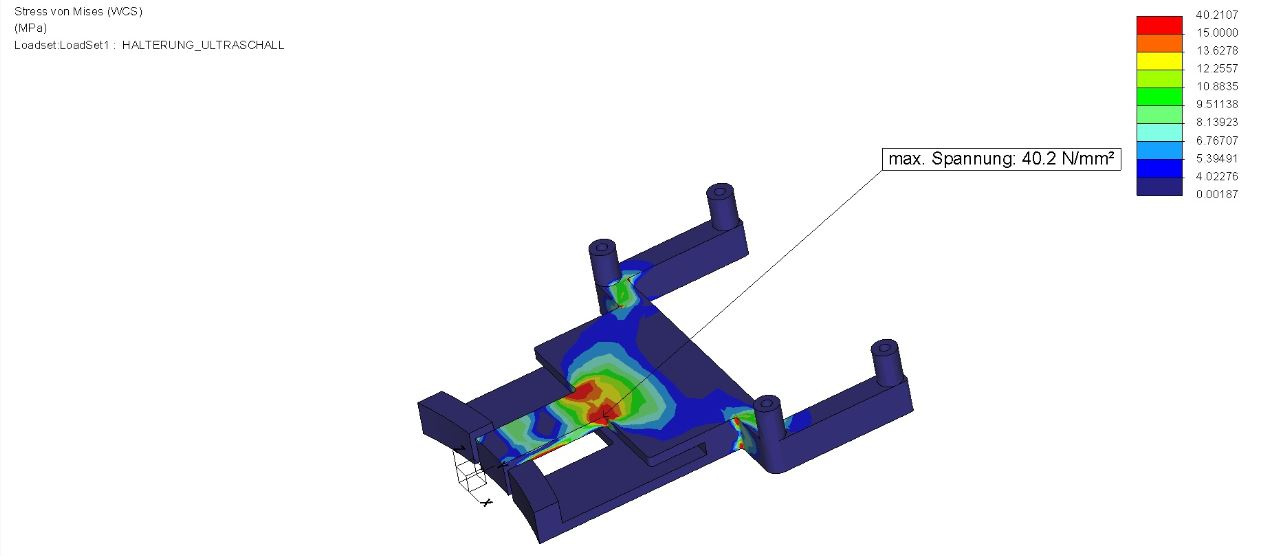
\includegraphics[width = 0.4\textwidth]{Bilder/max_spannung_f20_r0_5}}
						\subfigure[max. Spannung bei 20 N unten\label{max_spannung_f20_r0_5_oben}]{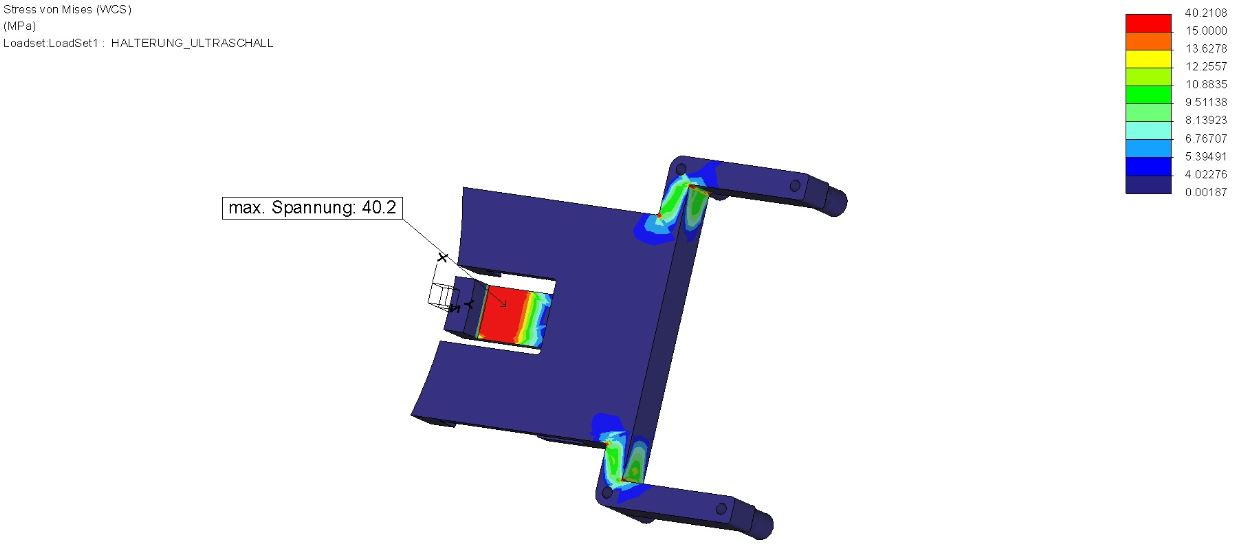
\includegraphics[width = 0.4\textwidth]{Bilder/max_spannung_f20_r0_5_oben}}
					\par\end{centering}
					\caption{max. Spannung bei 20 N}
					\label{max_spannung_f20_r0_5}
				\end{figure}

	Die maximale Spannung beträgt etwa 40.2 N, vergleicht man dies mit dem Ausschnitt aus dem Datenblatt (siehe Abbildung \ref{werte_abs}) sieht man,
	dass die maximale Biegespannung an beiden Stellen überschritten wurde. In der Realität würde das bedeuten, dass die Lasche bei dieser Belastung sehr stark verformt oder gar gebrochen wäre.
	Solche starken Beanspruchungen treten in diesem Fall niemals auf, da  bei einem Absturz die Halterung geschützt wäre.

	Um auch im Notfall hohe Belastungen kompensieren zu können, wurden in den Kanten der Laschen Rundungen vorgesehen. Den Zweck dieser Rundungen zeigen die folgenden Abbildungen.

			\begin{figure}[H]
				\begin{centering}
					\subfigure[max. Spannung bei 20 N, Radius 0.5 mm\label{max_spannung_f20_r0_5}]{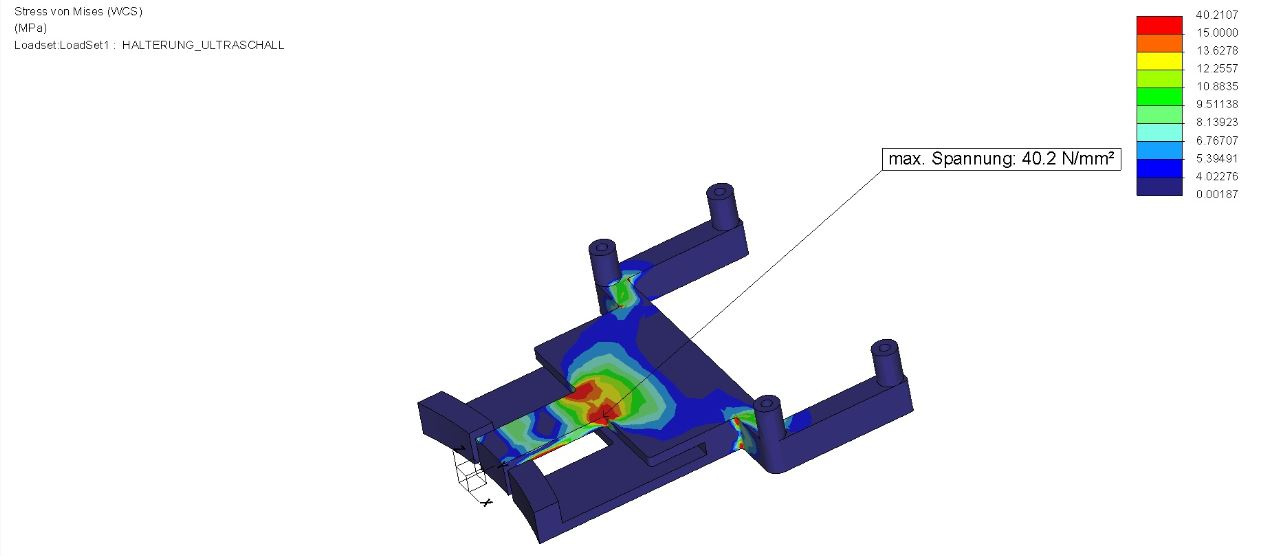
\includegraphics[width = 0.4\textwidth]{Bilder/max_spannung_f20_r0_5}}
					\subfigure[max. Spannung bei 20 N, Radius 1.0 mm\label{max_spannung_f20_r1}]{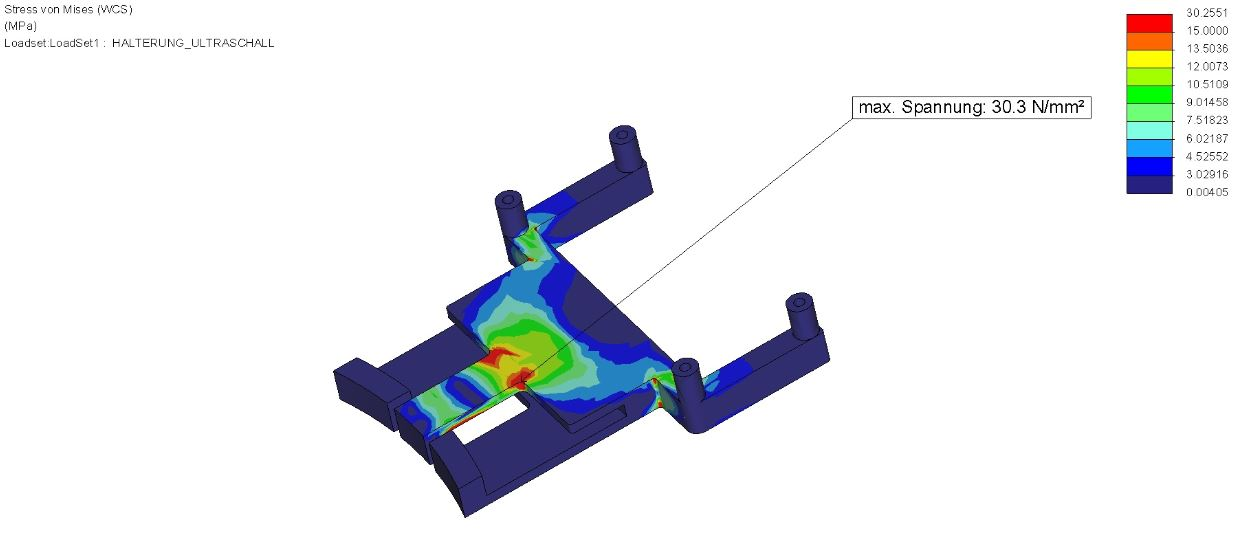
\includegraphics[width = 0.4\textwidth]{Bilder/max_spannung_f20_r1}}
				\par\end{centering}
				\caption{max. Spannung bei 20 N, unterschiedliche Radien}
				\label{max_spannung_f20_r0_5}
			\end{figure}

	Abbildung \ref{max_spannung_f20_r0_5} zeigt die Beanspruchung von 2 kg und einem Radius von 0.5 mm.
	Das Ergebnis zeigt, wie schon erwähnt, dass die maximale Biegespannung überschritten wurde.
	Abbildung \ref{max_spannung_f20_r1}, zeigt das Ergebnis mit der gleichen Kraft, aber einem Radius von 1 mm, also doppelt so groß wie in der ersten Simulation.
	Man kann sehr gut erkennen, dass die Spannung von 40.2 N/mm^{2} auf 30.3 N/mm^{2} gesunken ist, also um fast das eineinhalb-fache.

	Dieses Vorkommen wird in der Mechanik als \uline{Kerbwirkung} bezeichnet:




			\newpage

\section{Halterung PIXY CMU cam5}

	\subsection{Technische Planung}

	Der Hexacopter soll dem Gast sein gewünschtes Dessert bringen, der Weg zu dem Gast wird über Farbcodes am Boden vorgegeben.
	Um dem Farbcode folgen zu können, wird eine PIXY CMU cam5 verwendet (genaueres siehe Kapitel Sensoren).

	Die Halterung soll so konstruiert werden, dass die Kamera während des Fluges nicht wackelt, das verhindert ungenaue \bzw falsche Messwerte.
	Besonders zu beachten ist, dass die PIXY Cam immer in die Flugrichtung ausgerichtet sein muss.
	Der Flightcontroller gibt dem Hexacopter eine fixe Orientierung vor, würde die Kamera nicht in diese Richtung messen, könnte es zu Fehlmessung kommen und den Multicopter falsch navigieren.

	\subsection{Umsetzung}

	In den folgenden Abbildungen wird einerseits die konstruierte Halterung Abbildung \ref{halterung_pixy_creo})
	und andererseits die Gefertigte  mit der PIXY CMU cam5 (Abbildung \ref{halterung_pixy}).

			\begin{figure}[thb]
				\begin{centering}
					\subfigure[CAD Konstruktion PIXY Cam Halterung\label{halterung_pixy_creo}]{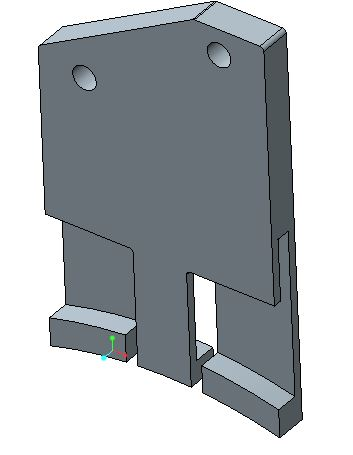
\includegraphics[width = 0.3\textwidth]{Bilder/halterung_pixy_creo}}
					\subfigure[Gefertigte PIXY Cam Halterung\label{halterung_pixy}]{\includegraphics[width = 0.4\textwidth]{Bilder/halterung_pixy}}
				\par\end{centering}
				\caption{Halterung PIXY Cam}
				\label{Halterung_PIXY}
			\end{figure}

	Aus Gewichtsgründen wurde die Halterung in einem 3D Drucker angefertigt.
	Diese wiegt etwa 5.2 g, ist also etwas leichter als die Ultraschallsensorhalterung.
	Um den Hexacopter, selbst bei so geringen Massen besser ausgleichen zu können, wurden beide Befestigungsmöglichkeiten gegenüber voneinander platziert.
	Da die PIXY Cam Halterung auf der unteren Centerplate platziert wird, konnte wieder das eigens entwickelte Klammersystem verwendet werden.
	Das garantiert auch in diesem Fall eine gute Passgenauigkeit, um den Sensor optimal zu fixieren.

	Die Kamera hat an der unteren Leiste der Platine zwei Bohrungen vorgesehen, diese wurden genutzt um den Sensor mit der Halterung zu verbinden.
	Es bot sich nicht viel Platz auf der Platine an, um den Sensor fest genug zu fixieren, jedoch reichte der untere Streifen ausreichend aus.

	Wie schon in der technischen Planung erwähnt wurde, spielt die exakte Position der PIXY Cam eine wichtige Rolle.
	Die Vorgangsweise zur Ermittlung der Ausrichtung wird mit der folgenden Abbildung erklärt.

			\begin{figure}[tbh]
			\begin{centering}
			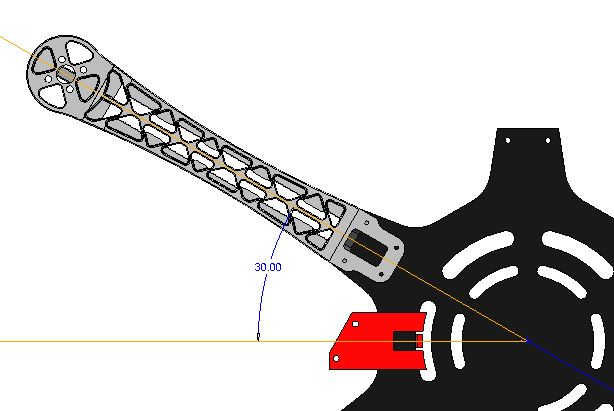
\includegraphics[width = 0.8\textwidth]{Bilder/winkel_pixy}
			\par\end{centering}
			\caption{Messung Winkel}
			\label{winkel_pixy}
			\end{figure}

	Der Flightcontroller wurde so eingebaut, dass ein Arm des Hexacopters zur Kontrolle in die Flugrichtung steht.
	Die \textcolor{red}{Halterung} wurde genau in der Mitte der Strebe platziert, daher konnte eine Konstruktionslinie vom Mittelpunkt der Platte aus, gesetzt werden.
	Der Winkel konnte gemessen werden, indem die zweite Konstruktionslinie entlang der Mitte des Arm gesetzt wurde.
	Die Schräge ist deshalb notwendig, da der Platz auf der Platine des Sensors so begrenzt ist, dass nur die Fläche der unteren Leiste aufliegen kann.

	\subsection{Herausforderungen und Lösungen}

	Der begrenzte Platz zum Montieren der PIXY Cam an der Halterung war die größte Herausforderung.
	Das  Problem war, dass sich auf der Platine eine Kabelbuchse befindet, diese ist genau auf der Ecke des Streifens vorgesehen (siehe Abbildung \ref{PIXY_Cam_Hinterseite}, orange markierter Bereich).

			\begin{figure}[H]
			\begin{centering}
			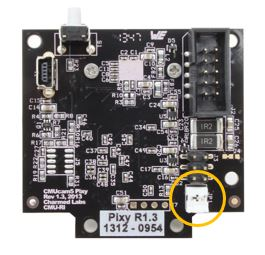
\includegraphics[width = 0.5\textwidth]{Bilder/PIXY_Cam_Hinterseite}
			\par\end{centering}
			\caption[PIXY Cam Anschlussbuchse]{PIXY Cam Anschlussbuchse\cite{PIXY_Cmu_cam5}}
			\label{PIXY_Cam_Hinterseite}
			\end{figure}

	In den Konstruktionen wurde dieses Problem nicht behandelt, erst bei dem ersten Test hat sich gezeigt, dass die Halterung nicht komplett passt.
	Um nicht noch eine neue Version drucken und Zeit verlieren zu müssen, wurde die Kante an der linken Bohrung (siehe Abbildung \ref{halterung_pixy_creo}) passgenau mit einer Feile abgerundet.

			\newpage

\section{Führung für Testflüge}

	\subsection{Technische Planung}

	Im Laufe des Projektes hat es sich bestätigt, dass es manchmal passieren kann, dass die Funkverbindung zwischen der Fernbedienung und dem Flugobjekt abbrechen kann.
	Ist jedoch keine Sicherung in der Firmware des Copters vorgesehen, fliegt dieser unkontrollierbar und stürzt ab.

	In diesem Projekt ist das Problem aufgetreten während eines Testfluges zur Testung der Höhenbestimmung durch den Ultraschallsensor.
	Damit dies nicht mehr vorkam, müsste eine Hardwaremäßige Vorrichtung entwickelt werden, die im Falle eines unvorhergesehenen Funkabbruches den Hexacopter sicher auf den Boden sinken lässt.

	\subsection{Umsetzung}

	Die folgende Abbildung zeigt die konstruierte (Abbildung \ref{gleitbuchse_creo}) und die gefertigte Gleitbuchse (Abbildung \ref{gleitbuchse_gefertigt}).

			\begin{figure}[tbh]
				\begin{centering}
					\subfigure[CAD Konstruktion Gleitbuchse\label{gleitbuchse_creo}]{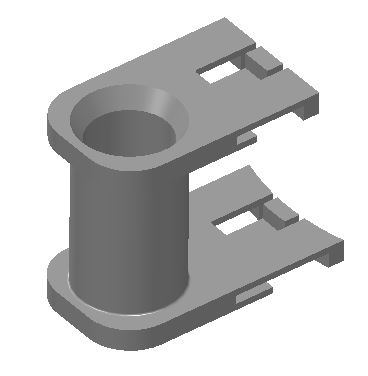
\includegraphics[width = 0.3\textwidth]{Bilder/gleitbuchse_creo}}
					\subfigure[Gefertigte Gleitbuchse\label{gleitbuchse_gefertigt}]{\includegraphics[width = 0.4\textwidth]{Bilder/gleitbuchse_gefertigt}}
				\par\end{centering}
				\caption{Gleitbuchse}
				\label{Gleitbuchse}
			\end{figure}

	Prinzipiell werden zwei Gleitbuchsen gegenüberliegend am Hexacopter montiert, der Copter wird dann auf zwei langen Stangen aufgefädelt und kann sich dadurch nur mehr nach oben und unten bewegen.
	Das soll verhindern, dass der Hexacopter nicht nach links, rechts, vorne oder hinten abdriften kann.
	Beide Buchsen verwenden das spezielle Klammersystem um sie leicht und fest montieren zu können, wie auch die Halterungen für den Ultraschallsensor und die PIXY Cam, werden die Führungen auf die Platte geklippt.
	Die Führungen wurden diesmal auf beide Centerplates befestigt, das bedeutet die obere Klammer musste an die Centerplate angepasst werden.
	Die Centerplates haben komplett verschiedene Ausnehmungen vorgesehen, das erschwerte die Anpassung des Klammersystems um ein Vielfaches.
	Um diese Herausforderung trotzdem lösen zu können, wurden die Platten in Creo ausgemessen und dann auf die Halterungen übertragen.

	Gefertigt wurden beide Teile in dem 3D Drucker der Schule, da die Form der Gleitbuchsen händisch sehr aufwändig zu fertigen werden würden, \bzw es wird sehr viel Gewicht durch diese Fertigungsmethode eingespart.
	Zu beachten war beim Konstruieren wiederum, dass der Drucker grobe Toleranzen hat und diese miteingerechnet werden mussten.

	Die Bohrungen wurden so groß dimensioniert, dass der Hexacopter leicht auf und ab fliegen kann, ohne zu stark zu verkanten.
	Die Phasen bei den Bohrungen oben und unten, lassen den Copter leichter auffädeln, da die Stangen leichter in die Bohrungen führen.

	\subsection{Herausforderungen und Lösungen}

	Das Verkanten zwischen den Buchsen und Stangen war besonders während des Startes ein Problem.
	Der Hexacopter hob zu Beginn etwas  schief ab, das kann man auch nicht mit sehr großen Bohrungen verhindern.
	Es musste manuell mit der Fernsteuerung entgegen dieses Neigens gesteuert werden, damit der Multicopter abheben konnte.
	Nach etwa 5 cm hatte sich der Copter so ausgeglichen, dass nicht mehr entgegen gesteuert werden musste.
	Die Gleitbuchsen haben sich trotzdem sehr bewährt, da der Multicopter, auch wenn er kein Gas mehr gab, nur auf dem Landesgestell landete und so keine Teile beschädigt wurden.

			\newpage

\section{Persönliche Erfahrungen}

	\subsection{Abteilungsübergreifendes Arbeiten}

	Die Erfahrung, dass man ein Projekt Klassen,- oder gar Abteilungsübergreifend umsetzt, ist für die Vorbereitung im Berufsleben sehr wichtig.
	Es besteht ein großer Unterschied, ob man in einer Gruppe arbeitet, die man jeden Tag in der Klasse trifft, oder in einem Team, welches man nur zu Meetings oder kurzen Gesprächen sieht.
	Dieses Problem haben wir nicht nur durch die Jour fixes, sondern auch mit den KaTeCos (alle drei Wochen) gelöst.
	Die KaTeCos waren besonders wichtig, da nicht nur der Projektverlauf im Detail besprochen wurde, sondern auch die Teamfähigkeit gestärkt wurde.

	\subsection{Arbeiten im allgemeinen}

	Die Vorgangsweise zur Umsetzung eines Teiles war meist die gleiche, eine Idee, eine Konstruktion in Creo und die Fertigung im 3D Drucker.
	Im Laufe des Projektes hat sich herausgestellt, dass die Planung \bzw die Anhaltspunkte zur Konstruktion am wichtigsten waren.
	Das hat sich beim Entwickeln des Rotorschutzes gezeigt, die Planung wurde vernachlässigt in Creo angefangen zu zeichnen.
	Die Folge war, dass dieses Ziel ins Stocken kam und immer mehr Zeit auf sich genommen hat.
	Nachdem der Rotorschutz nahezu aussichtslos schien, begann ich mich mit den Halterungen für die Sensoren zu beschäftigen,
	diese „Abwechslung“ hat dazu geführt, dass neue Ideen zur Optimierung des Propellerschutzes entstanden, welche dann auch zum Abschluss des Zieles führten.

	\subsection{Arbeiten mit dem 3D Drucker}

	Der 3D Drucker der Schule ist eine faszinierende Maschine, es kann fast jedes Teil präzise anfertigen, egal welche Form es hat.
	Wir hatten das Glück diesen Drucker verwenden zu dürfen \bzw wurden sogar von EVO-tech mit Druckmaterial unterstützt.
	Es war besonders bei den Halterungen sehr komfortabel, dass wir diese drucken konnten. Das Klammersystem könnte nur sehr mühsam gefertigt werden, es müsste sogar eine andere Lösung gefunden werden.

	Man muss sich an jede Maschine die man verwendet erst gewöhnen, man lernt wie man sie bedienen muss, ihre Probleme und Makeln.
	Der Evolizer ist ein hoch entwickeltes Produkt, jedoch muss man auch hier die richtige Bedienung kennenlernen.
	Es hat sich zum Beispiel herausgestellt, dass der Drucker erst eine gewisse Temperatur braucht, bis das Filament auf der Platte haftet, oder dass der Abstand zwischen der Platte und Düse sehr genau eingestellt gehört.
	Durch solche Probleme lernt man, wie man mit der Maschine umgehen muss und wie man sie optimal bedient, diese Erfahrung kann im weiteren Berufsleben sehr essenziel sein.

	\subsection{Zusammenfassung}

	Zusammenfassend ist zu sagen, dass die Diplomarbeit eine sehr wichtige Erfahrung und Lehre ist.
	Man lernt so viel Neues kennen, mit dem man gar nicht rechnen würde, zum Beispiel neue Programme zum optimierten und leichteren Arbeiten oder Managementmethoden die die Planung übersichtlicher und trotzdem detailliert gestalten.

 	In unserem Fall war es noch so, dass wir uns fast kaum kannten und dennoch erstaunliche Erfolge feiern konnten,
	das beweist, dass man sich nicht unbedingt kennen muss um ein gutes Projekt realisieren zu können. Solche Erfahrungen können besonders in der Berufslaufbahn genutzt werden,
	da man immer wieder mit einem Team arbeitet, welches man vielleicht nicht so gut kennt.


\include{Testphase_Erfahrungen_Ergebnisse}

\renewcommand{\kapitelautor}{}
\appendix

\chapter{Anhang 1\label{chap:Anhang-1}}

\printindex{}

\bibliographystyle{plaindin}
\bibliography{diplom}


%%%%%%%%%%%%% GLOSSAR teil 2/2 - muss getestet werden
\printglossary[type=\acronymtype]
\printglossaries


\end{document}
